\documentclass[dvipdfmx, 12pt]{article}
\usepackage{mathpazo}
\usepackage{amsmath,amssymb}
\usepackage{array}
\usepackage[hiresbb]{graphicx}
\usepackage{tikz}
\usepackage{textcomp}
\usepackage{dcolumn}
\usepackage{here}
\usepackage{lscape}
\usepackage[top=25truemm,bottom=30truemm,left=25truemm,right=25truemm]{geometry}
\begin{document}

\title{Reference Dependence and Monetary Incentive \\
-Evidence from Major League Baseball-}
\author{Reio Tanji}
\date{}
\maketitle

\leftskip = 25pt
\rightskip = 25pt
  \small
  \textit{
  Many empircal studies have revealed the existance of reference-point dependent preference in field settings, including cases from professional sports players' decision making, whose performance is observed by the manager and is evaluated as their monetary rewards. If there are some incentives, or discontinuities in their rewards that encourage individuals to take behavior that ``appears'' to be driven by the reference dependence, we should the conclude that it is caused by the design of the contracts. In this paper, we picked up a case of Major League Baseball players, whom Pope and Simonsohn (2011) reported have reference-point dependent preferences about the number of their batting-average. Then, we confirmed the evidences of manipulation in batting-average and other performance indexes, and tested if there existed any monetary incentives that encouraged the players to do so. We found three implications: first, there actually existed manipulation in the players' batting-average. Second, surprisingly, there were little evidences that supported the monetary-incentive hypothesis. Third, among the variable indexes, .300 of batting-average was a solid benchmarks for the playrs.
  }

\leftskip = 0pt
\rightskip = 0pt
\normalsize


\section{Introduction}

Reference-point dependence is one of the most important concepts to evaluate outcomes, and it affects agents' following economic behavior. Classical economic models assume that economic agents evaluate their choices/prospects according to the abolute value of (expected) return. On the other hand, Tversky and Kahneman (1992) introduced the behavioral assumption: reference-point dependent preference consider outcomes by the relative value to some target value of the outcomes, reference points. That is, subjects regard the possible outcome as gain or loss from the target. For example, workers feel happy if her/his wage goes up to \$15 per hour, but vice versa if it goes down to \$15, although the absolute value of \$15 is actually the same. In this case, s/he evaluates their new wage with the reference point of the previous one.

In this paper, we explore whether players play only for monetary rewards or they play to reach their target because otherwise they incur disutility, using data on individual performance indexes in Major League Baseball (MLB).

Prospect theory consists of two main characteristcs: one is the probability weighting function, and the other is the reference dependence, mentioned above. It enabled us to interpret phenomena that cannot be explained by the traditional microeconomic theory. Thus,we observe that many following researches have been conducted in field and laboratory settings.

Reference dependence also also in the behavior of athletes. Pope and Schweizer (2011) found that professional golf players regarded ``per,'' the standard number of shots determined according to the difficuly of each hole, as reference points. Additionally, Allen et al. (2016) argued that marathon runners adjusted their finish times just before the round number times (just three or four hours), the reference points. Similarly, Pope and Simonsohn (2011) showed the existance of the reference point in the MLB, a professional baseball league of the U.S.

MLB position players evaluate themselves by the indexes that measure their performance. Moreover, they seems to have some reference points in their self-evaluation, for example, about their batting performance indexes: .300 of batting average. Pope and Simonsohn (2011) have shown that there exists bunching just above .300 of the distribution of this index.

Pope and Simonsohn (2011) differs from the former two papers, however, because players receive monetary rewards determined according to their performance.

Consider the case of the professional golf player. Golf is essentialy competition of the total number of shots they needed to finish the whole tour, regardless of that of each single hole, or whether s/he saves par or not in the hole. The rank of order is determined according to the total number of shots, and those with better scores are rewarded. Then, there appears a question that what if there is some monetary incentive to make effort to save per. In other words, suppose when every time s/he saves par in each hole, s/he can get some additional bonus separated from their total score. In this case, then, making effort to save par can be interpreted as sufficiently ``rational'' choice for the player, although the observed behavior itself appears to be evidence of the reference dependence. However, there usually does not exist any additional monetary rewards such as ``Save-Par-Bonus.''

On the contrary, in MLB,, it might not be sufficient to prove that the bunching is caused by reference point dependent utility function about their performance indexes: team managers may assign some monetary incentives for the players to adjust their aspiration level to meet those points, as we described in the example above.

Our most important contribution of this paper is to reveal the observed behavior to be in fact reference dependence. There are two things to be mentioned. First, we confirmed the evidence for the manipulation of the performance indexes around the round numbers, by using McCrary (2008)'s method to test manipulation. We include analysis of not only .300 of batting average but also other points of batting-average and other indexes, such as homerun or stolen-bases. Second, we explored whther this observed manipulation was truly driven by the reference dependence of the players. We applied regression analysis using the data of the players' salary.

Our paper found three important results. First, our examination for manipulation supported Pope and Simonsohn (2011). We observed there  existed seemingly reference point dependent behavior, where .300 of batting-average worked as a reference point. Similar results were obtained about other round numbers of batting-average, and other batting indexes such as on-base percentage or homerun. Second, we found that as a whole, there did not exist any monetary incentive for them: for their fixed part of the salary contract, we conclude their monetary rewards are continuous at just above the each performance index, such as .300 of batting-average. That is, they behave as they consider these round numbers as reference points, even though they does not receive any additional payment by achieving them. Furthermore, we reinforce our results, discussing some alternative interpretation about other types of monetary incentives: the part of incentivesed contract, and relation with contract length. Finally, there exists serial changes about the players' index manipulation. .250 of batting-average does not work as a reference point in relatively recent years, while 20 of homerun does only in the recent players. Among them, .300 of batting-average seems to be a solid benchmarks for the players.

This paper proceed as follows. In the Section 2, we review some literature and verify the standpoint of my paper. Section 3 describes the data we availed. Section 4 presents theoretial framework and empirical  specification, and make some conjecture.  Section 5 shows the results of the analysis. Discussion about some alternative interpretation and non-statistical data are included in Section 6. Finally, Section 7 provide concluding remarks.

\section{Literature Review}

  Tversky and Kahneman (1992) mentioned reference point dependence as one of the two distinct respects of their prospect theory. The most primitive form of reference dependent utility function is:

   \[
  u(x | r) = \begin{cases}
  x - r & \text{ if }x \geq r \\
  \lambda (x - r) & \text{ if }x < r
\end{cases}
  \]
  where $x$ denotes a certain outcome, and $r$ is one of the reference points (Figure \ref{gain-loss}). This agent evaluates the outcome by a difference from the reference point. In adiition, they assume ``loss-aversion'' of the individual, or $\lambda > 1$. %Those who have this type of utility function, than they regard same absolute amount of outcome in different way, depending on s/he faces gain or loss situation.%
  ``Diminishing sensitivity,'' which is concave in facing gain and convex in facing loss is an advanced form of this specification (Figure \ref{dim-sen}).

  Diecidue and Van de Ven (2008)`s ``aspiration level'' model added discontinuity assumption: that is, a utility function that ``jumps'' at the reference point (Figure \ref{jump}). When there exists jump in their utility function, then individuals try to manipulate their outcome level, paying addtional cost which is not incorporated into the model with the standard continuous utility function. As a result,  excess mass or bunching around or just above the reference point arises. We discuss the required functional assumptions of them in Section 4.1.

  Individuals with such reference-point dependent utility try to put their effort so as to achieve their internal target, or reference point. There is a number of empirical literature that specifies the existence of reference dependence in the field or lab experimented studies. Farber (2008) applied this model to the labor supply of New York cab drivers to show that as soon as they reached daily target sales, they quit, even when they reached it early in each day. Jones (2018) analyzed on the system of American tax payment. He showed that individuals tried to manipulate their real payment by substituting it by donation or other charitable action, and that especially when facing losses, they put more effort. This observation is also caused by the feeling of loss-aversion, with the reference point of zero-payment threshold.

  \begin{tabular}{ccc}
    \begin{minipage}[H]{0.3\textwidth}
      \begin{figure}[H]
        \begin{tikzpicture}
          [domain = -2:2, samples = 200, >= stealth]
          \draw[->] (-2,0) -- (2,0) node[right]{$x$};
          \draw[->] (0,-2) -- (0,2) node[above]{$u(x)$};
          \draw plot[domain = 0:1.7] (\x, \x);
          \draw plot[domain = -0.9:0] (\x, {2 * \x});
          \draw (0,0) node [below right] {$r$};
        \end{tikzpicture}
        \scriptsize
        \caption{primitive gain-loss function}
        \label{gain-loss}
      \end{figure}
      \end{minipage} &
      \begin{minipage}[H]{0.3\textwidth}
        \begin{figure}[H]
          \begin{tikzpicture}
            [domain = -2:2, samples = 200, >= stealth]
            \draw[->] (-2,0) -- (2,0) node[right]{$x$};
            \draw[->] (0,-2) -- (0,2) node[above]{$u(x)$};
            \draw plot[domain = 0:1.7] (\x, {sqrt( \x)});
            \draw plot[domain = -1.7:0] (\x, {-sqrt(2 * - \x)});
            \draw (0,0) node [below right] {$r$};
          \end{tikzpicture}
          \scriptsize
          \caption{diminishing sensitivity}
          \label{dim-sen}
        \end{figure}
        \end{minipage}&
        \begin{minipage}[H]{0.3\textwidth}
          \begin{figure}[H]
            \begin{tikzpicture}[domain = 0:4, samples = 200, >= stealth]
              \draw[->](-0.5, 0) -- (4.2, 0) node[right]{$x$};
              \draw[->](0, -0.5) -- (0, 3.7) node[above]{$u(x)$};
              \draw[-](2.2, -0.1) -- (2.2, 0.1);
              \draw[domain=0:2.2,samples=200,>=stealth] plot (\x, {sqrt(\x)});
              \draw[domain=2.2:4.1,samples=200,>=stealth] plot (\x, {sqrt(\x) + 0.8});
              \draw (0, 0) node[below left]{O};
              \draw (2.2, -0.3) node {$r$};
            \end{tikzpicture}
            \scriptsize
            \caption{jump at the reference point}
            \label{jump}
          \end{figure}
        \end{minipage}
      \end{tabular}

\vspace{1zw}


Reference dependence also arises in the cases of sports. One of the most well-known papers among them is Pope and Schweizer (2011). They obtained the data of professional golf players, to point out that in each hole, players behave as they take ``par'' as the reference point. Specifically, they scceeed in their putts, significantly better when the putt was one to save par than when it was one to get ``eagle'' or ``birdie.'' Similarly, Allen \textit{et al} (2016) specified the existance of reference point dependence of marathon runners, using data of the finish time of enormous number of race in the United States. In this case, the distribution of finishing time has excess mass around evry 30 minutes. Note that these cases are common in that the outcomes themselves are nonmonetary ones, and even if they achieve their internal goals, they do not receive any additional monetary reward for their success. Professional golf players are awarded according to the total number of shots through the whole tour, not to the number of pers they saved.

Pope and Simonsohn (2011) mention a seemingly similar case. They picked up three empirical evidences of round numbers that work as reference points: SAT (a standardized test for college admission in the United States) scores, laboratory experiment, and baseball. In their section of baseball, they picked up the evidence of Major League Baseball (MLB) players. They argue that the players have reference dependent preference in evaluating themselves their perfonmance index: batting-average (AVG). According to their paper, the position players (batters) pay attention to their batting-average (AVG) especially to finish each season with their batting average of just above .300. They obtained MLB season individual AVG data from 1975 to 2008 and observed position players (= players except for pitchers) with at least 200 at-bats in each season. Then, they found that their distribution of the batting-average had excess mass just above .300, which reveals the existance of manipulation there. Furthermore, they found that players with batting-average of just below .300 were more likely to hit a base-hit and less likely to get a base-on-balls. Both base-hits and base-on-balls avoid the batter from being gotten out, so for the team which he belongs to, base-on-balls also have important value to win the game. However, batting-average does not count base-on-balls as an element to raise the number (For the definition of performance indexes, see Appendix), so they prefer getting hit to base-on-balls. %Thus, observed behavior they claims is sufficient evidence that shows the existance of round-number reference point dependent preference of the MLB players.%

There is similar behavior to the cases of  Allen \textit{et al} (2016): bunching. However, one important thing we have to take care of is that they are professional athlete, and so there exists procedure of contract between the player and the team manager: those who evaluate the player. They propose the players contracts for the next season, after observing the performance they had shown in this season. In other words, the observed excess mass may be derived by their monetary value function, not by the preference of themselves. We will distinguish them, which is the main contribution of this paper.

Pope and Simonsohn (2011) conducted analysis only for batting-average, and following research is to be made. So we first search for the round numbers of various batting indexes manipulated by the players. Then, we test if there exists any monetary incentives for the players. The team managaers and the players agree the contract that sets fixed additional bonuses which is paid when a certain performance index reaching to the point. For the players whose indexes are around the cutoff points, making discontinuously large effort, and the following observed bunching can be interpreted as economically rational choice, under the given the contract design.
%In general, players with their performance index just above these cutoff point and those just below the point have almost same ability as a baseball player. At least, it is natural to think there is no reason to treat players discontinuously better, only because he achieve the cutoff. Then, it is interpreted that it is rather the team manager than the players themselves who have the reference-point dependent preference, which makes the players encouraged to meet their goals. Also if such a type of evaluation is utilized, then the managers can get players that are as skilled as those with .300 of batting average, by relatively reasonable contracts.%

%On the other hand, if there exists no evidence that team managers evaluate the players by the achievement of the cutoff, then we can say that the observed behavior is truly drawn by their own reference dependence. In addition, the consistency is so strong that even there exists no rational reason, they try to reach there.

\section{Data Description}

To make empirical research, we need information about players' performance, contracts and other details. Then, we obtained panel data that contain these specific information from some open data-source. Each sample consists of indexes of a player at the end of a single season. Here we explain the specific information about the dataset.

First, Performance data are obtained from baseball fan website:  \textit{fangraphs} and \textit{Baseball References}. We collected information since 1957 season, the year when the qualified number of plate-appearances was regulated. It is the cutoff point to be eligible for the title of leading hitter, the player with the highest batting-average. Stats in each season covers only the regular season, not Spring-Training or postseason games. The full-sample is $N=54469$.

Note that we then restrict the sample to the players who appear to the plate in MLB games enough to be tested, because those with little number of plate-appearances are likely to be evaluated by other elements than their batting skills \ldots pitching or fielding, performance at the minor leagues, or those who injured at the season. Especially about batting-average and on-base percentage, those of players with few plate-appearances are not be regarded as reliable. Pope and Simonsohn (2011) set the cutoff at 200 of at-bats, but alternatively we use 200 plate-appearances as the required number to be considered in our analysis. This is because at-bat does not count the number of base-on-balls or sacrifice bunts in the denominator, even though they surely appear to the plate and made something to their teams. On the other hand, plate-appearance stands for the number of chances of batting their coaches gave him. Restricting the sample reduces the sample size to $N=18143$.

The dataset includes the players' plate-appearance, batting-average, on-base percentage, homerun, stolen-base, runs-batted-in, base-hit, all of them are the main indexes of interest in this paper. In addition, for the regression analysis, we obtain additional indexes: batting, fielding, and BaseRun, the estimated contribution to the team expressed in the runs they produced, and WPA, or winning percentage added. Further explanations used in our analysis are provided in Appendix.

We then describe the nature of the indexes. Baseball batting indexes are roughly divided into two types. The first is the one that simply indicates the number of a certain plays, and the second is the one calculated using these numbers, which indicates the rate or the expected number of the plays. Here we call the former ``cumulative index,'' and the latter ``rate index.'' Cumulative indexes are for example ``base-hit'' or ``homerun,'' or ``stolen-bases.'' Cumulative indexes are irreversible and so they are monotonically increasing in their appearances. That is, once the players reached a certain number of cumulative indexes such as 20 homeruns, it does not matter how their performance goes afterward. On the other hand, rate indexes can fluctuate: even once they reached their internal goals, it may fall if their performance get worse. Batting-average and on-base percentage are sorted to this type.

Second, we mention the salary data. Salary data are obtained from \textit{USA TODAY} and \textit{Baseball References}. We collected annual salary data of the position players who registered into MLB Roaster at the beginning of each season. They also contain information about other player-specific characteristcs: age, position (such as catcher, 1st-baseman, left-fielder, designated hitter and so on), the teams they signed, and the possession of free agency. We merged this dataset with the play stats in the previous year, because salary is usually determined based on the performance of the previous season. Because of lack of disclosed information, this dataset contains data on salary only from 1987. Also, because we regard the players' performance as reflected to their annual reward in that of the next year, we cannot merge the stats dataset of 2018. So the latast available season is 2017. The aggregated number of the panel is $N=13226$, and the restriction of 200 plate-appearances reduces the number to $N=8915$. Then, here we  use two datasets: one that contains salary data (we call this Sample B), while the other does not (Sample A). As we explain in the next section, we use two main analysis: manipulation of performance index (only use play stats) and design of the contracts (needs information about salary). In the former we use Sample A, and in the latter Samlple B. The descriptive statistics of each sample are descripted in Table 1 and Table \ref{sum_B}, respectively.

\begin{table}
  
% Table created by stargazer v.5.2.2 by Marek Hlavac, Harvard University. E-mail: hlavac at fas.harvard.edu
% Date and time: ��, 11 08, 2018 - 14:34:36
% Requires LaTeX packages: dcolumn
\begin{table}[H] \centering
  \caption{Summary Statistics for Sample A}
  \label{sum}
\scriptsize
\begin{tabular}{@{\extracolsep{1.2pt}}lD{.}{.}{-3} D{.}{.}{-3} D{.}{.}{-3} D{.}{.}{-3} D{.}{.}{-3} D{.}{.}{-3} D{.}{.}{-3} }
\\[-1.8ex]\hline
\hline \\[-1.8ex]
Statistic & \multicolumn{1}{c}{N} & \multicolumn{1}{c}{Mean} & \multicolumn{1}{c}{St. Dev.} & \multicolumn{1}{c}{Min} & \multicolumn{1}{c}{Pctl(25)} & \multicolumn{1}{c}{Pctl(75)} & \multicolumn{1}{c}{Max} \\
\hline \\[-1.8ex]
PA & 18,143 & 456.477 & 152.836 & 200 & 320 & 591 & 778 \\
HR & 18,143 & 11.811 & 9.747 & 0 & 4 & 17 & 73 \\
RBI & 18,143 & 51.882 & 26.912 & 4 & 31 & 69 & 165 \\
SB & 18,143 & 7.846 & 10.869 & 0 & 1 & 10 & 130 \\
AVG & 18,143 & .264 & .032 & .135 & .242 & .285 & .394 \\
OBP & 18,143 & .331 & .039 & .174 & .305 & .356 & .609 \\
Age & 18,143 & 28.506 & 4.042 & 18 & 25 & 31 & 46 \\
H & 18,143 & 108.941 & 42.933 & 29 & 72 & 143 & 262 \\
OPS & 18,143 & .738 & .106 & .382 & .665 & .805 & 1.422 \\
\hline \\[-1.8ex]
\end{tabular}
\end{table}

\end{table}

\leftskip = -15pt
\begin{table}
  
% Table created by stargazer v.5.2.2 by Marek Hlavac, Harvard University. E-mail: hlavac at fas.harvard.edu
% Date and time: ��, 11 08, 2018 - 14:49:25
% Requires LaTeX packages: dcolumn
\begin{table}[H] \centering
  \caption{Summary Statistics for Sample B}
  \label{sum_B}
\scriptsize
\begin{tabular}{@{\extracolsep{-5pt}}lD{.}{.}{-3} D{.}{.}{-3} D{.}{.}{-3} D{.}{.}{-3} D{.}{.}{-3} D{.}{.}{-3} D{.}{.}{-3} }
\\[-1.8ex]\hline
\hline \\[-1.8ex]
Statistic & \multicolumn{1}{c}{N} & \multicolumn{1}{c}{Mean} & \multicolumn{1}{c}{St. Dev.} & \multicolumn{1}{c}{Min} & \multicolumn{1}{c}{Pctl(25)} & \multicolumn{1}{c}{Pctl(75)} & \multicolumn{1}{c}{Max} \\
\hline \\[-1.8ex]
Age & 8,915 & 28.714 & 3.901 & 19 & 26 & 31 & 46 \\
PA & 8,915 & 471.946 & 150.890 & 200 & 342 & 605.5 & 778 \\
AVG & 8,915 & .268 & .031 & .146 & .248 & .289 & .394 \\
OBP & 8,915 & .337 & .038 & .174 & .311 & .360 & .609 \\
HR & 8,915 & 13.446 & 10.213 & 0 & 6 & 19 & 73 \\
RBI & 8,915 & 56.339 & 27.621 & 5 & 35 & 74 & 165 \\
SB & 8,915 & 8.534 & 10.851 & 0 & 1 & 11 & 109 \\
H & 8,915 & 114.232 & 42.481 & 30 & 78 & 148 & 262 \\
+WPA & 8,915 & 8.715 & 3.471 & 2.030 & 5.820 & 11.430 & 19.160 \\
-WPA & 8,915 & -8.270 & 2.610 & -15.050 & -10.420 & -6.060 & -2.740 \\
Bat & 8,915 & 3.257 & 16.139 & -44.200 & -7.300 & 11.100 & 116.800 \\
Fld & 8,870 & .304 & 7.482 & -36.100 & -4.000 & 4.400 & 37.000 \\
BsR & 8,915 & .092 & 2.712 & -12.600 & -1.200 & 1.200 & 14.300 \\
Salary & 8,915 & 3,487,838 & 4,487,344 & 62,500 & 512,750 & 4,658,334 & 29,200,000 \\
FA & 8,915 & .168 & .374 & 0 & 0 & 0 & 1 \\
\hline \\[-1.8ex]
\end{tabular}
\end{table}

\end{table}
\leftskip = 0pt

\section{Theoretical Frameworks and Way of Specification}

\subsection{Frameworks}

Many sports are so rich in performance indexes that record plays in variable viewpoints. Among them, especially, baseball performance indexes can distribute individual-separatable evaluation to the players, not only evaluating performance by units of the whole team. Thus, baseball performance indexes are interpreted as reliable proxies for the skills of the players. Here we assume that the players are trying to maximize them, with their internal costs depending on their talented skills. After observing the indexes the players generated, team managers evaluate them and propose contracts of the next year (also, they include the player-specific characteristcs: age, position and so on). Then, the players' monetary rewards are given by the following function:

\[
F_{it+1} = F(X_{it}, Z_{it})
\]
where $F$ stands for the monetary reward function to the player $i$ at time $t+1$, and $X_{it}$ and $Z_{it}$ express the value of the index and other player characteristcs, respectively. The player makes decision on his effort to maximize their utility, according to this benefit function.

On the other hand, another inpretation is that each player evaluates himself as an athlete: he directly yields utility by his value of the performance indexes. That is, players make decision making according to their utility function

\[
U_{it} = U(X_{it})
\]
In this model, the player no longer pays attention to his future monetary rewards similar to the first model, and he decides his effort level to maximize his utility.

It is nnoted that we cannot determine which model is appropreate to interpret the observed behavior of the players: excess mass or bunching around the possible referene points. If the players' own reference dependent preferences about the performance indexes cause them,  then $U(.)$ has functional features that represent reference dependence. On the other hand, if their contracts designed to lead them to the bunching around some possible reference point, now we can regard that $F(.)$ has the features described. Our interest is that which of the two assumptions are in fact observed.

Then, we consider the functional features of $F(.)$ or $U(.)$, which cause bunching of the histgrams of the indexes. In this paper, we avail the two models quated in Section 2: one is ``kink'' at the reference point, and the other is ``notch'' of the function.

\begin{enumerate}
  \item \textbf{``notch'' at $r$} (Figure \ref{notch})

  The first possible assumption is discontinuity at a certain cutoff point of the function, described as follows:

  \begin{align*}
    \lim_{\epsilon \to 0} U_r (r + \epsilon) & \neq
    \lim_{\epsilon \to 0} U_r (r - \epsilon) \\
    \lim_{\epsilon \to 0} F_r (r + \epsilon) & \neq
    \lim_{\epsilon \to 0} F_r (r - \epsilon)
  \end{align*}
  This is the discontinuous form of the function at the cutoff point $r$, introduced by Diecidue and Van de Ven (2008).

  \item \textbf{``kink'' at $r$} (Figure \ref{kink})

  \begin{align*}
    \lim_{\epsilon \to 0} U'_r (r + \epsilon) & \neq
    \lim_{\epsilon \to 0} U'_r (r - \epsilon) \\
    \lim_{\epsilon \to 0} F'_r (r + \epsilon) & \neq
    \lim_{\epsilon \to 0} F'_r (r - \epsilon)
  \end{align*}

  $U'(.)$ and $F'(.)$ stand for the first-order differential of $U(.)$ and $F(.)$, respectively ($U(.)$ and $F(.)$ are assumued to be continuous differential). As we explained in the Section 2, this is the primitive form of reference dependence, introduced in Kahneman and Tversky (1979) and Tversky and Kahneman (1992).
\end{enumerate}

\begin{tabular}{cc}
  \begin{minipage}[H]{0.5\textwidth}
    \begin{figure}[H]
      \begin{tikzpicture}[domain = 0:4, samples = 200, >= stealth]
        \draw[->](-0.5, 0) -- (4.2, 0) node[right]{$X$};
        \draw[->](0, -0.5) -- (0, 3.7) node[above]{$F(X), U(X)$};
        \draw[-](2.2, -0.1) -- (2.2, 0.1);
        \draw[domain=0:2.2,samples=200,>=stealth] plot (\x, {sqrt(\x)});
        \draw[domain=2.2:4.1,samples=200,>=stealth] plot (\x, {sqrt(\x) + 0.8});
        \draw (0, 0) node[below left]{O};
        \draw (2.2, -0.3) node {$r$};
      \end{tikzpicture}
      \scriptsize
      \caption{"notch" at the reference point}
      \label{notch}
    \end{figure}
    \end{minipage} &
    \begin{minipage}[H]{0.5\textwidth}
      \begin{figure}[H]
        \begin{tikzpicture}
          [domain = -2:2, samples = 200, >= stealth]
          \draw[->] (-2,0) -- (2,0) node[right]{$X$};
          \draw[->] (0,-2) -- (0,2) node[above]{$F(X), U(X)$};
          \draw plot[domain = 0:1.7] (\x, \x);
          \draw plot[domain = -0.9:0] (\x, {2 * \x});
          \draw (0,0) node [below right] {$r$};
        \end{tikzpicture}
        \scriptsize
        \caption{"kink" at the reference point}
        \label{kink}
      \end{figure}
    \end{minipage}
\end{tabular}

\vspace{2zw}

Allen \textit{et al.} (2016) also supposed these types of model, and specified bunching of the marathon runners' finish time around the round numbers. Both two possible assumptions result in bunching at the cutoff point: in our paper, we consider these cutoffs are the round numbers of the performance indexes, such as .300 of batting-average. Therefore, we regard it as not so important that which of the two to be appropreate to describe the bunching itself: that is, our interest is whether $F(.)$ has these types of functional features in the number of performance indexes. In words, the players salary scheme might be designed so that players make effort to meet their cutoff points. In the rest of this subsection, we explain the possible design of the contracts.

\vspace{1zw}

Let us consider the first case: monetary reward ``jumps'' at the possible reference point. Then, the salary function is decomposed into two terms as follows.

\[
F_{it+1}(.) = f(X_{it}, Z_{it}) + D_{it} \textit{Bonus}(X_{it})
\]

$f(.)$ is determined by the the number of the performance index $X$ and other player-specific characteristcs $Z$, note that this term is continuous in $X$. $D$ is the dummy variable that depends on $X$: to indicate whether the player's index is above the cutoff point. If the players achieve the cutoff point like .300 of batting-average, then $F$ discontinuously rise by the appearance of $\textit{Bonus}$ term. And as a result, salary scheme with this form of function cause the excess mass around the cutoff, by the players who desire the additional monetary rewards.

The second case, on the other hand, express the ``kink'' of $F$ as follows:

\[
F_{it+1}(.) = (1-I_{it})g(X_{it}, Z_{it}) + I_{it}h(X_{it}, Z_{it})
\]

$I$ is the same indicator as $D$, which takes 1 if $X$ is larger than the cutoff, 0 otherwise. There are two salary schemes depending on the players performance index, represented by $g$ and $h$. $g$ is applied for the players with the index below the cutoff, and $h$ is for those with above there. Furthermore, $h$ consists of two terms: $h(.,.) = g(c, Z{it}) + k(X_{it}-c)$. $c$ stands for the given cutoff. In words, players receive continuous reward in their performance index, but the return to them changes after they achieve the cutoff: in our assumption, decrease. More directly, the marginal rate of return to their performance index discontinuously diminishes: kinks at the reference point.

If the observed bunching is because of the contract design, then the salary scheme has at least one of the features above. In the next section, we describe how to specify them.

 \subsection{Empirical Method}

  \subsubsection{Test for Bunching}

  First, we test if there is observed any behavior that seems to be related to reference dependent preference. As we explained in the previous sections, manipulation is verified by the observation of bunching, or an excess mass around the possible reference point. To specify the excess mass, we apply the method of regression discontinuity design (RDD).

  RDD is a way to measure the effect of a treatment, such that whether the treatment is assigned or not depends on the threshold of a certain variable (called ``running variable''). Then, comparing the samples just above and just below the threshold is sufficient examination of the treatment, since they are in almost same states except for the existance of the treatment.

  However, there is an important assumption for this specification to be valid (Lee and Lemieux, 2010): continuity of the running variable around the threshold. In other words, individuals must not be able to manipulate the running variable so as to be above the cutpoint. This is because if there exists manipulation, then there occurs selection bias problem, that those who try to be assigned the treatment can adjust their running variable. Therefore, there are some empirical way to test the manipulation of a variable, which is the very method I apply in our analysis. One of the frequently applied methods for this specification is  McCrary(2008)'s local linear density estimation. We avail this to our specification of bunching.

  This test of the manipulation at the cutoff point $c$, proceeds in two steps. First, define $f(.)$ be the density function of the variable $x$ to be tested (here we use the performance indexes). Then we undersmooth the observed density: determine the binsize $b$ of $x$, and obtain the histgram. And finally, we conduct local linear approximation to both just above and below the cutoff point. Note that the optimal bandwidth is to be selected by the fourth order polynominal approximation. Then, we estimate the frequency at the cutoff point, $\Hat{f}(r)$, by fitting the estimated density function from both below and above the cutoff, $\hat{f}^+$ and $\hat{f}^-$, respectively. Finally, we take the difference between $\ln \hat{f}^+$ and $\ln \hat{f}^-$ to calculate the statistics $\theta$. With $\theta$ and its estimator of standard deviation, $t$-tests can be conducted to specifying manipulation.

  \subsubsection{Monetary Incentive}

  Then, We examine the existance of the monetary incentive. For this procedure, the specification of the two functional features mentioned in Section 4.1 is to be required: notch and kink at a certain cutoff points.

  First, we specify the salary scheme $F(.,.)$ with notch at the cutoff. Here we exploit the linear function, that is,

  \[
  F(X_{it}) = w_{it} = \beta_0 + \beta_1 \text{PERF}_{it} + \beta_2 \text{ABOVE}_{it}
  \]
  For each player $i$ in the season $t$, $w_{it}$ is loggarithm of their annual salary in next season $t+1$. $\text{Performance}_{it}$ is the value of performance index (batting-average, on-base percentage,\ldots), described as $X_{it}$ in Section 4.1. $\text{ABOVE}_{it}$ is an indicator of the achievement of their goals for the index, which corresponds to $D$ in Section 4.1. If the estimated value of $\beta_2$ is supported to be positive and significant, then we consider there is an additional bonus paid to the player that reached a certain target value of the performance index, which leads them to bunching.

  On the other hand, the second possibility, the kink at the reference point is specified as follows.

  \[
  F(X_{it}) = w_{it} = \beta_0 + \beta_1 \text{PERF}_{it} + \beta_2 \text{ABOVE}_{it} + \beta_3 \text{PERF}_{it} \times \text{ABOVE}_{it}
  \]

  The first, second and the third terms are same as specification of notch, the linear salary scheme in the performance index. In addition, we introduce the interaction term of $\text{PERF}_{it}$ and $\text{ABOVE}_{it}$. This term stands for the return to the performance index for the players that achieve the cutoff point. In words, players with .320 of batting-average, for example, are evaluated by $\beta_1$ until .300, and then $\beta_1 + \beta_3$ for the rest .020 (it is the case of that bunching at .300 is argued). If the estimated value of $\beta_3$ is negative and significant, then there exists kink in the reward function, which again support the bunching at the cutoff point.

  Then, we describe the empirical specification. In our paper, we specify the linear functions described above by the regression analysis, for each performance index (batting-average, for example) and cutoff point (.300). We apply the methodology of regression discontinuity design (RDD). That is, we restrict the sample to those who are around the cutoff of each index. The bandiwidths in each analysis are selected according to the optimization of Imbens and Kalyanaraman (2009), using polynominal approximation. For the same bandwidth, we also conduct regression with the interection term of $\text{PERF}_{it}$ and $\text{ABOVE}_{it}$ to see the kink at the reference point.

  Furthermore, to check the robustness of the results, we include the terms about the player-specific characteristics as well, which correspoids to $Z_{it}$, mentioned in Section 4.1. Thus, the model to be estimated is:

  \begin{align*}
    w_{it} & = \beta_0 + \beta_1 \text{PERF}_{it} + \beta_2 \text{ABOVE}_{it} + \mathbf{b} \mathbf{Z}_{it} \\
    w_{it} &= \beta_0 + \beta_1 \text{PERF}_{it} + \beta_2 \text{ABOVE}_{it} + \beta_3 \text{PERF}_{it} \times \text{ABOVE}_{it} + \mathbf{b} \mathbf{Z}_{it}
  \end{align*}

  We employ OLS in each estimation and team and individual fixed effect models are also included.

  Note that we have to consider the possibility of endogeneity problem about our results. We discuss this in Section 5.

\section{Result}
\subsection{Excess Mass Around The Reference Point}

In this section, we present our main results of analysis. First, we show the results that verify bunching. Table \ref{Bunch-True} includes the summary of McCrary (2008)'s manipulation tests about the performance indexes showing that there is some manipulation occurs. Consistent with Pope and Simonsohn (2011), there actually exists excess mass around .300, and in addition .250 of batting-average. Manipulation was also observed in some of other round numbers of other indexes: .350 of on-base percentage, 20 of homeruns, 100 of runs-batted-in, 30 and 40 of stolen-bases, and 200 of base-hits.

\begin{table}
  \small
  \centering
  \begin{tabular}{lcccccc}\hline
    index & type & cutpoint & binsize & bandwidth & $\theta$ & $z$
    \\ \hline \hline
    AVG & rate & .300 & .001 & .019 &  .499 & 7.442*** \\
    & & & & & (.067) & \\
    & & .250 & .001 & .024 & .212 & 5.061*** \\
    & & & & & (.042) & \\
    OBP & rate & .350 & .001 & .024 &  .139 & 2.854** \\
    & & & & & (.049) &  \\
    HR & cumulative & 20 & 1 & 5.309 & .259 & 3.465*** \\
    & & & & & (.075)  & \\
    RBI & cumulative & 100 & 4 & 15.423 & .311 & 3.295*** \\
    & & & & & (.094) & \\
    SB & cumulative & 30 & 1 & 10.000 & .529 & 4.274*** \\
    & & & & & (.124) & \\
    & & 40 & 1 & 11.505 & .481 & 2.764** \\
    & & & & & (.174) & \\
    PA & cumulative & 500 & 1 & .003 & .160 & 2.515* \\
    & & & & &(.063) & \\
    H & cumulative & 200 & 1 & 18.922 & .453 & 2.547 * \\
    & & & & & (.178) & \\ \hline \hline
    Note & \multicolumn{6}{r}{
    ***: $p<0.1\%$, **: $p<1\%$, *: $p<5\%$.
    }\\
    \multicolumn{7}{r}{
    Bandwidth is optimized following the method of McCrary(2008).
    }
  \end{tabular}
  \caption{Test for Manipulation, leastPA $= 200$}
  \label{Bunch-True}
\end{table}

\begin{figure}
  \centering
  \begin{tabular}{ccc}
    \multicolumn{2}{c}{
    \begin{minipage}{.5\textwidth}
      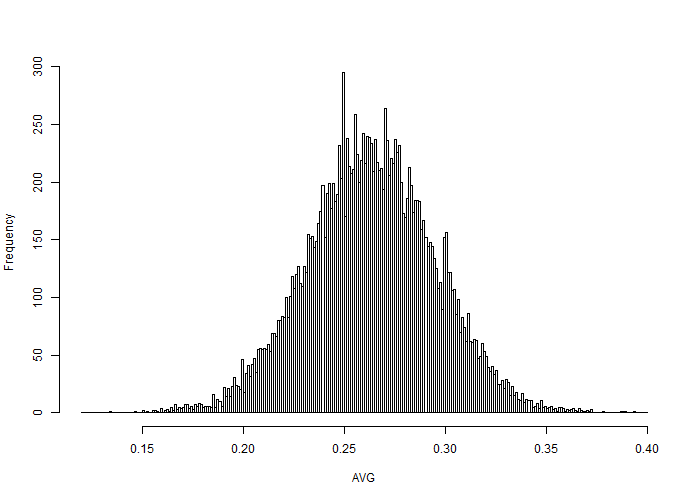
\includegraphics[keepaspectratio, scale = 0.5, angle=0]{graphs/hist_AVG_all.png}
      \caption{Histgram of Batting-Average}
      \label{}
    \end{minipage}
    } \\
    \multicolumn{1}{l}{
    \begin{minipage}{.4\textwidth}
      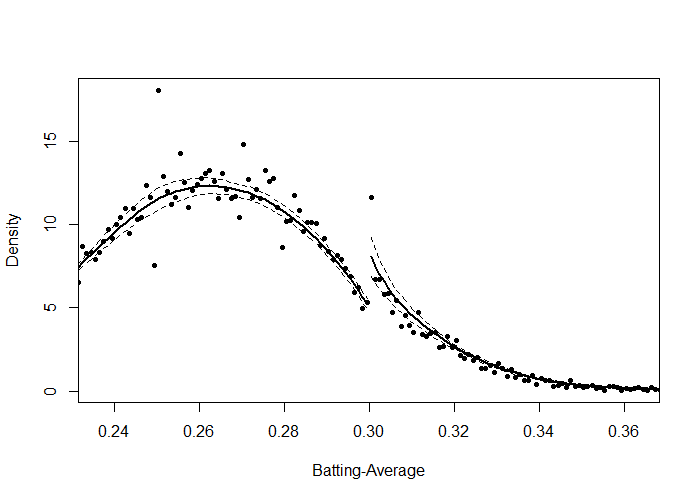
\includegraphics[keepaspectratio, scale = 0.5, angle = 0]{graphs/AVG_300.png}
      \caption{Discontinuity at .300 of AVG}
      \label{DCdensity_AVG_300}
    \end{minipage}
    } & &
    \multicolumn{1}{r}{
    \begin{minipage}{.4\textwidth}
      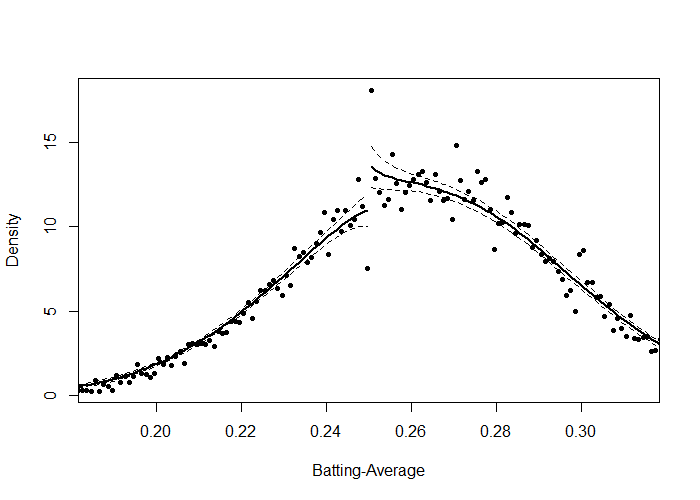
\includegraphics[keepaspectratio, scale = 0.5, angle = 0]{graphs/AVG_250.png}
      \caption{Discontinuity at .250 of AVG}
      \label{DCdensity_AVG_250}
    \end{minipage}
    }
  \end{tabular}
\end{figure}

\begin{figure}
  \centering
  \begin{tabular}{lr}
    \begin{minipage}{.5\textwidth}
      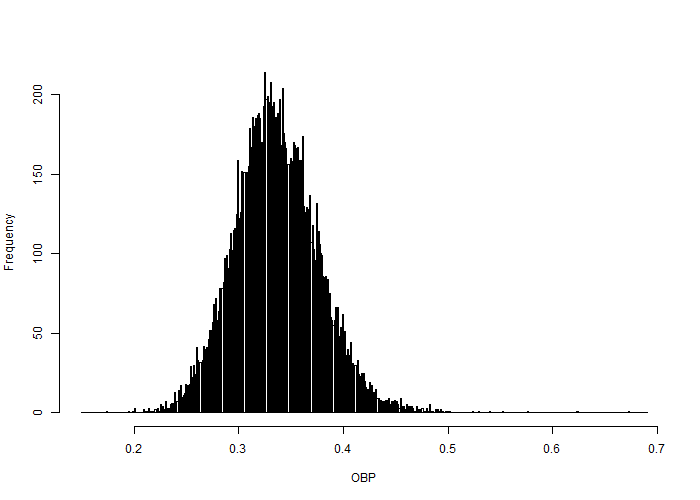
\includegraphics[keepaspectratio, scale = 0.3, angle=0]{graphs/hist_OBP_all.png}
      \caption{Histgram of On-Base Percentage}
      \label{hist_OBP}
    \end{minipage} &

    \begin{minipage}{.5\textwidth}
      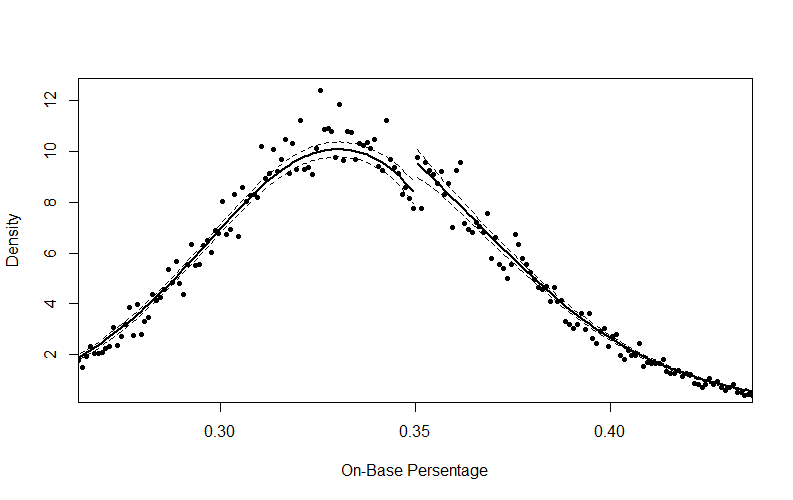
\includegraphics[keepaspectratio, scale = 0.4, angle = 0]{graphs/OBP_350.png}
      \caption{Discontinuity at .350 of OBP}
      \label{DCdensity_OBP_350}

    \end{minipage} \\

    \begin{minipage}{.5\textwidth}
      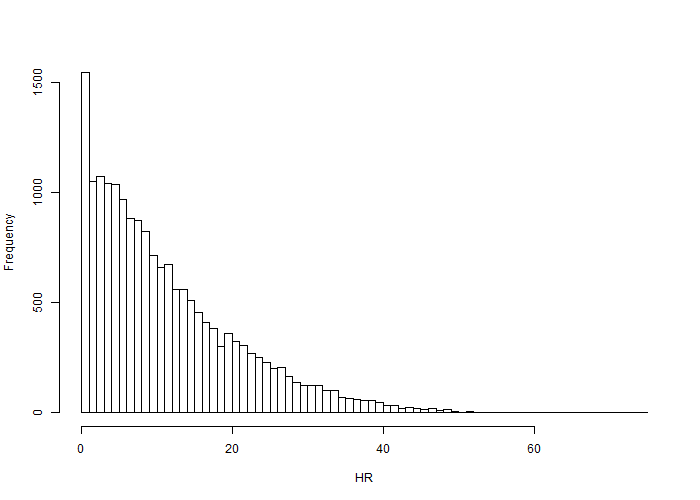
\includegraphics[keepaspectratio, scale = 0.3, angle=0]{graphs/hist_HR_all.png}
      \caption{Histgram of Homerun}
      \label{hist_HR}
      \end{minipage} &

      \begin{minipage}{.5\textwidth}
        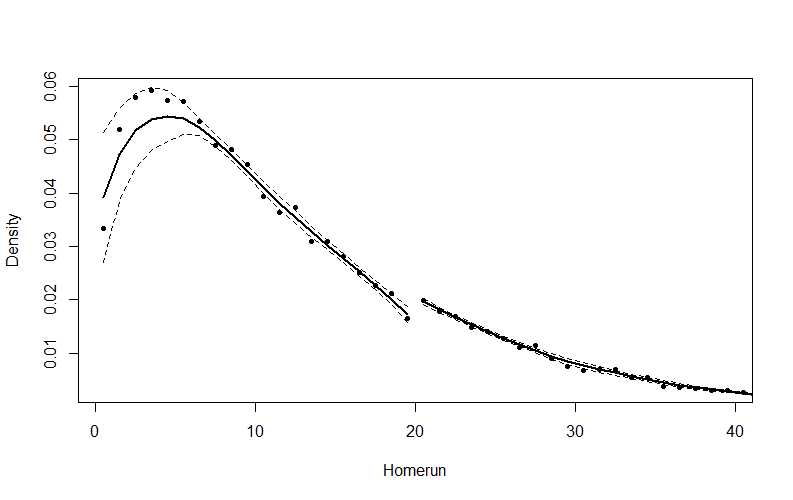
\includegraphics[keepaspectratio, scale = 0.4, angle = 0]{graphs/HR_20.png}
        \caption{Discontinuity at 20 of HR}
        \label{DCdensity_HR}

    \end{minipage}
  \end{tabular}
\end{figure}

\begin{figure}
  \centering
  \begin{tabular}{cc}
    \begin{minipage}{.5\textwidth}
      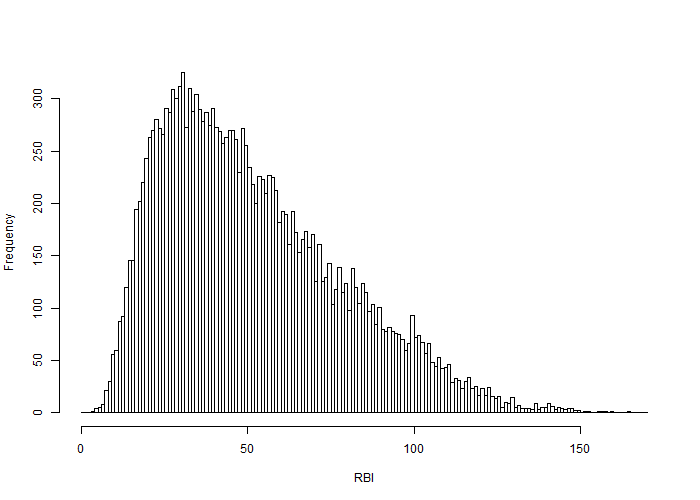
\includegraphics[keepaspectratio, scale = 0.3, angle=0]{graphs/hist_RBI_all.png}
      \caption{Histgram of Runs-Batted-In}
      \label{hist_RBI}
      \end{minipage} &

      \begin{minipage}{.5\textwidth}
        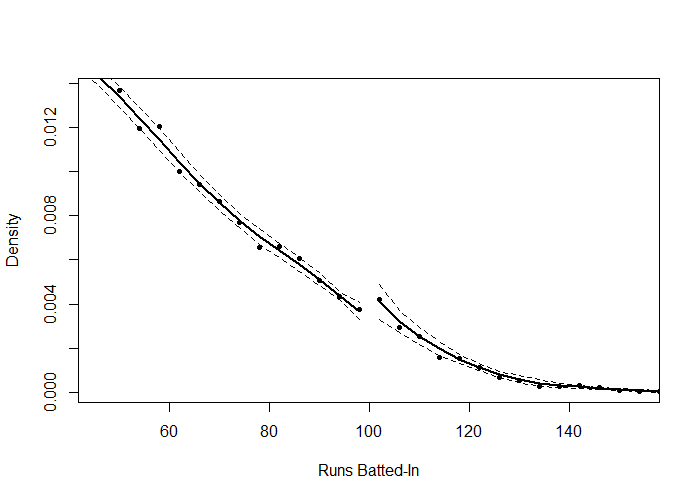
\includegraphics[keepaspectratio, scale = 0.4, angle = 0]{graphs/RBI_100.png}
        \caption{Discontinuity at 100 of RBI}
        \label{DCdensity_RBI_100}

      \end{minipage} \\

      \begin{minipage}{.5\textwidth}
        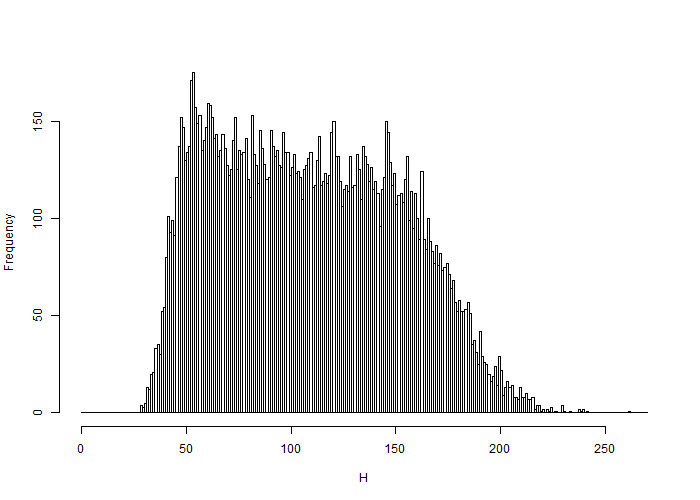
\includegraphics[keepaspectratio, scale = 0.3, angle=0]{graphs/hist_H_all.png}
        \caption{Histgram of Base-Hit}
        \label{hist_H}
      \end{minipage} &

      \begin{minipage}{.5\textwidth}
        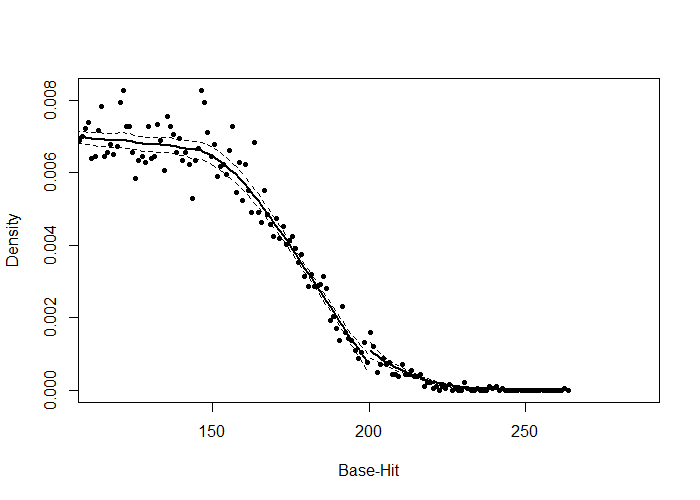
\includegraphics[keepaspectratio, scale = 0.4, angle = 0]{graphs/H_200.png}
        \caption{Discontinuity at 200 of Base-Hit}
        \label{DCdensity_H_200}

      \end{minipage}
  \end{tabular}
\end{figure}

\begin{figure}
  \centering
  \begin{tabular}{ccc}
    \multicolumn{2}{c}{
    \begin{minipage}{.5\textwidth}
      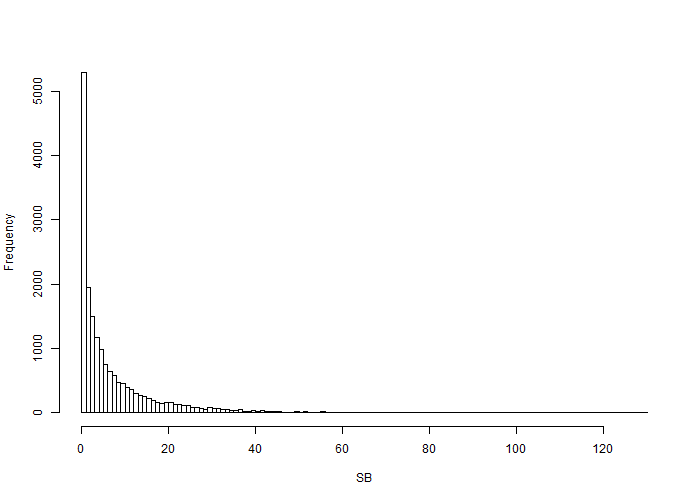
\includegraphics[keepaspectratio, scale = 0.5, angle=0]{graphs/hist_SB_all.png}
      \caption{Histgram of Stolen-Base}
      \label{hist_SB}
    \end{minipage}
    } \\
    \multicolumn{1}{l}{
    \begin{minipage}{.4\textwidth}
      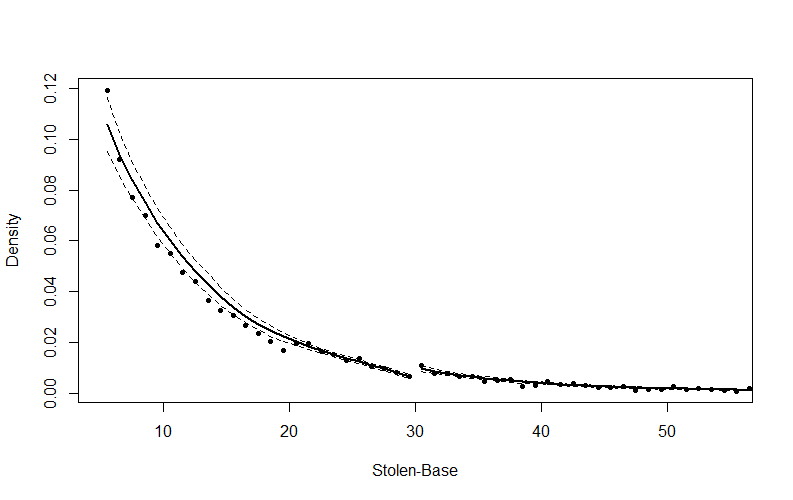
\includegraphics[keepaspectratio, scale = 0.5, angle = 0]{graphs/SB_30.png}
      \caption{Discontinuity at .300 of AVG}
      \label{DCdensity_SB_30}
    \end{minipage}
    } & &
    \multicolumn{1}{r}{
    \begin{minipage}{.4\textwidth}
      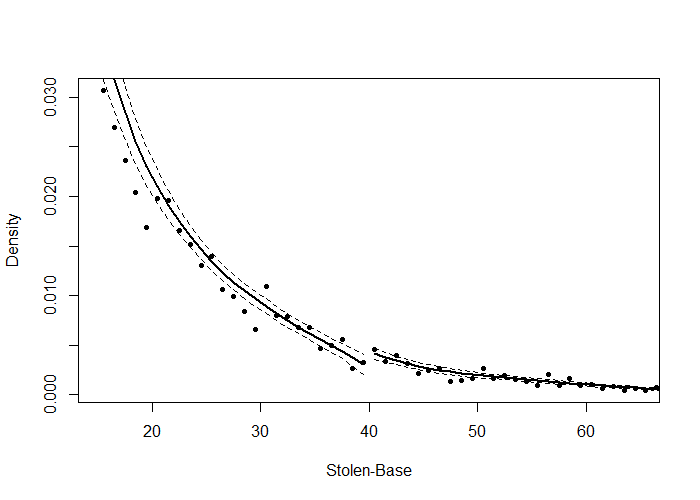
\includegraphics[keepaspectratio, scale = 0.5, angle = 0]{graphs/SB_40.png}
      \caption{Discontinuity at .250 of AVG}
      \label{DCdensity_SB_40}
    \end{minipage}
    }
  \end{tabular}
\end{figure}

For precise estimation of bunching, we set the binsizes of undersmoothing artificially: .001 for batting-average and on-base percentage, 1 for homerun (HR), stolen-base (SB), plate-apparance (PA), and base-hit (H), and 4 for runs-batted-in (RBI). Batting-average (AVG) and on-base percentage (OBP) are usually shown by three decimal digits, rounding the fourth decimal digit, so strictly batters with .2995 of batting-average are taken as .300. As we mentioned in Section 3, homerun, stolen-base, plate-appearance, and base-hit stand for the number of plays in interest, and they therefore take integer and they earn one for each plate appearance. Runs-batted-in is also an integer-index, but it can get at most 4 at one plate-appearance, so we set it 4. To confirm the robustness of our results, we repeated this test with various binsize, but we yield essentialy the same results. Bandwidths are optimized by calculation, following McCrary (2007).

For .300 of batting-average, when we increased the sample size compared with Pope and Simonsohn (2011), we obtained similar results: Players puto effort to manipulate their batting-average. The difference between the estimated frequency according to the approximation below .300 and that of above .300 was significant at the .1\% ($z=7.442$) level.

In addition, bunching occurs in .250 ($z = 5.061$, $p < .1\%$) as well. It was not reported in Pope and Simonsohn (2011): there was no bunching observed in any other round numbers of batting-average, so bunching may have occurred in before 1973 (Pope and Simonsohn (2011) includes dataset after 1974). We specifically analyzed this in Section 6.4. Replicating analysis with larger binsizes: .002 and .005 also yields similar results.

On-base percentage, on the other hand, showed similar tendency in .350, at the significance level was the 5\% level ($z=2.854$). Pope and Simonsohn (2011) reported that they were less likely to get base-on-balls when their batting-average was just below .300 at the last plate-appearance of the season. This attitude is in one respect tradeoff to raise on-base percentage, so we can consider that players feel that batting-average is more important than on-bace percentage. Observed results however, support the excess mass about on-bace percentage as well.

Bunching also occurs in cumulative indexes. Cumulative indexes have different nature from the rate indexes, as we mentioned in the previous sections, but they showed basically similar results. Similarly to batting-average and on-base percentages, this bunching is observed only in limited numbers, not in all the round numbers. For Homerun, bunching occurrs only in 20 ($z=3.465, p < 0.1\%$): there may be diminishing sensitivity: 20 is located on above the 75 percentiles of the whole Sample A. We observe bunching also at 30 ($z=4.274, p < 0.1\%$) and 40 ($z=2.764, p < 1\%$) of stolen-base and 200 in base-hit ($z=2.547, p < 5\%$). Stealing-bases require skills that are talented to limited number of the players, but succeeds with the prpbability of 60\% to almost 100\%, so those who are evaluated by their number of stolen-bases can manipulate them. 30 and 40 of stolen-bases are also far above the 75 percentiles of all the players.

Base-hit is also manipulated, but the confidence level of the discontinuity was lower than that of batting-average ($z$ = 2.547, $p < 5\%$). Base-hit is an index close to batting-average, because both indexes increase by getting base-hits. We obtain this result because the number of base-hit is not regarded as important as batting-average (In most TV live on baseball, they introduce player with his batting-average, not the number of base-hits.) Alternatively, we can consider that this is the difference between the cumulative indexes and the rate ones. If a player reaches .300 of batting-average, for example, then he can keep it by not attending the rest of plate-appearances or games. In fact, Pope and Simonsohn (2011) pointed out that players with just above .300 were more likely to be replaced their last sceduled plate-appearance. On the other hand, if he get the 200th base-hit, then he does not have to care about the number of base-hits and attend the games to get better performance.

Surprisingly, such manipulation occurs in runs-batted-in ($z$=3.295, $p$<0.1\%), too. Compared to other indexes, runs-batted-in is harder to manipulated, because the number of that depends on the performance of his teammates, and the number they can earn at a single plate-appearance varies from 1 to 4. As in Table \ref{Bunch-True}, there occurs the evidence in plate-appearances. However, it may not be convincing because the optimized bandwidth was smaller than one, even though the number of PAs takes only integers. Setting bandwidth larger than 1, then the result turned out to be insignificant, so we regard it as not supportive results for bunching. (In fact, there certainly exists monetary incentives for plate-appearances. We come back to here in Section 6.1.)

Summarizing the results, there in fact exists excess mass or bunching at the some round numbers of the batting indexes and they are possible reference point of the players. In the case of marathon runners, Allen et al. (2016), there occured bunching in every round numbers of the goal time, although the size of discontinuity decreased. That is, it should be considered that the reference points are not determined only by round numbers as argured by Pope and Simonsohn (2011) argued. That is, the nature of the reference points are likely to be close to ``par'' in Pope and Schweizer (2011), or the well-known standards that is related to the image of ``skilled players,'' rather than round numbers; or well, these numbers are monetarily incentivised goals by the team managers. So next, we examine whether there is any monetary bonus in their contract.

\subsection{Existance of Monetary Incentive}

In Section 5.1, we confirmed the discontinuities at the cutoff points of the representative indexes. Then in this section, we show whther they are led to aim these goals by their reference dependence, or by their design of the contracts with monetary incentive.

Table \ref{RDD_A} describes the results of local linear regression on loggarithm of their salary next year, with the cutpoint of each possible reference point. Column ``Other Control'' indicates if the model includes other player-specific variales (Deffence, BaseRun, player's age, WPA and dummy for possession of the right of free agency) and season dummies. ``bw type'' indicates the bandwidths used in the model: ``LATE'' includes the sample that are in the optimal bandwidth calculated by Imbens and Kalyyanaraman (2009), while ``Half-BW'' and ``Double-BW'' are using a half and a twice of the LATE bandwidth, respectively. As a whole, there is no evidence that suports the existance of monetary incenive to make effort for their observed goals. There is no essential difference between the cumulative indexes and rate indexes. That is, the reward function $F(.,.)$ does not discontinuously jump at each cutoff points.

Also, we made regression analysis with an interaction term of $X_{it}$ and $\text{ABOVE}_{it}$, which considers the change in average return of the index in argument to their annual salary when the value of the index is above the cutoff point. This model corresponds to specifying kinks at the possible reference points. Table \ref{AVG300_A} to \ref{SB40_A} show the results of this regression for each cutoff point, respectively. Results again denied existance of monetary incentives for bunching, they give us no evidence of neither kink or jump of their reward functions. Here we consider each indexes respectively.

First, for batting-average, results denied the existance of any additional monetary bonus for achieving either .300 or .250. Although estimated jump at each cutoff points were positive, but their standard errors are large and so the difference were insignificant at the 5\% level. The same results were obtained in the model with interaction terms (Table \ref{AVG300_A} and \ref{AVG250_A}): the estimated coefficients of the dummies for achieving their internal goals and the interaction term with the batting-average are all insignificant. That is, the monetary reward does not discontinuously jump or kink at .300 of .250. These findings are consistent with the hypothesis that preferences of the players are reference dependent about their batting-average and excess mass is caused by them, not by the monetary incenitves.

On-base percentage shows similar tendency. The estimated jump takes negative, although the estimator is insignificant. Also, by Table \ref{OBP350_A}, negative kink is not observed. On-base percentage is considered as relatively more important index: it is closer correlation with the winning-average of the team than batting-average. Thus, it can be the case that team managers evaluate on-base percentage more than batting-average and think of paying players with higher number more. However, our results are against this hypothesis.

Also for the cumulative indexes, observed results are almost the same: 20 of homerun, 100 of runs-batted-in, and 200 base-hits work as the cutoff points of bunching, but not as the marginal poits for the players' salary. Homeruns produce at least one score to the team, and are take one of the most ``attractive'' aspects of baseball, so there may exists additional positive effect for the team: it may bring a lot of audience, which profits them by stadium fees. Nevertheless, discontinuous scheme of the salary was not observed. Regressions with the interaction term does not report kink at each cuttoff point.

\begin{table}[H]
  \caption{RDD Test for Monetary Incentives}
  \label{RDD_A}
  \fontsize{9pt}{6pt}\selectfont
  \centering
  \begin{tabular}{@{\extracolsep{0pt}}lccccccc}\hline
    index,cutpoint & Other Control & bw type & bandwidth
    & Observations & Estimate & Std. Error & $z$
    \\ \hline \hline
    AVG, .300 & No &LATE & .084 & 8514 & .047 & .061 & .773 \\
    & &Half-BW &  .042 & 5599 & .088 & .075 & 1.174 \\
    & & Double-BW & .170 & 8915  & .067 & .056 & 1.184 \\ \cline{3-8}

    & Yes &LATE & .045 & 5930 & .034 & .056 & .615 \\
    & &Half-BW &  .023 & 3005 & .061 & .077 & .788 \\
    & & Double-BW & .090 & 8605  & .016 & .045 & .354 \\ \hline

    AVG, .250 & No &LATE & .036 & 6110 & .019 & .068 & .286 \\
    & &Half-BW &  .018 & 3496 & .015 & .092 & .161 \\
    & & Double-BW & .072 & 8539  & .034 & .054 & .636 \\ \cline{3-8}

    & Yes &LATE & .048 & 7271 & .070 & .052 & 1.340 \\
    & &Half-BW &  .024 & 4402 & .066 & .069 & .953 \\
    & & Double-BW & .096 & 8810  & .075 & .044 & 1.713 \\ \hline

    HR, 20 & No & LATE & 3.32 & 1315 & .071 & .175 & .406 \\
    & & Half-BW & 1.66 & 562 & .073 & .127 & .576 \\
    & & Double-BW & 6.64 & 2582 & -.004 & .109 & -.034 \\ \cline{3-8}

    & Yes & LATE & 3.30 & 1307 & -.002 & .141 & -.015\\
    & & Half-BW &1.65 & 560 & .030 & .102 & .299 \\
    & & Double-BW & 6.61 & 2558 & -.032 & .088 & -.364 \\ \hline

    OBP, .350 & No &LATE & .044 & 6440 & -.038 & .065 & -.592 \\
    & & Half-BW & .021 & 3542 & -.076 & .089 & -.849 \\
    & & Double-BW & .087 & 8656 & -.029 & .051 & -.570 \\ \cline{3-8}

    & Yes & LATE & .045 & 6525 & -.013 & .049 & -.272 \\
    & & Half-BW & .022 & 3673 & -.055 & .069 & -.807 \\
    & &Double-BW & .089 & 8637 & .004 & .039 & .107 \\ \hline

    RBI, 100 & No & LATE & 4.08 & 393 & .072 & .289 & .250 \\
    & &Half-BW & 2.04 & 228 & .282 & .400 & .707 \\
    & &Double-BW & 8.16 & 714 & .008 & .185 & .043 \\ \cline{3-8}

    & Yes & LATE & 4.04 & 390 & .018 & .209 & .086 \\
    & & Half-BW & 2.02 & 227 & -.042 & .324 & .130 \\
    & & Double-BW & 8.07 & 708 & .056 & .127 & .435 \\ \hline

    H, 200& No & LATE & 3.173 & 75 & -.786 & .396 & -1.985* \\
    & & Half-BW & 1.587 & 35 & .386 & .271 & -1.421 \\
    & & Double-BW & 6.347 & 137 & -.061 & .309 & -.199 \\ \cline{3-8}

    & Yes & LATE & 3.175 & 75 & -.420 & 1.042 & -.403 \\
    & & Half-BW & 1.587 & 35 & -4.779 & .576 & -8.288** \\
    & & Double-BW & 6.349 & 137 & -.109 & .413 & -.265 \\ \hline

    SB, 30 & No & LATE & 3.39 & 282 & .962 & .372 & 2.585** \\
    & &Half-BW & 1.70 & 134 & .920 & .263 & 3.492*** \\
    & &Double-BW & 8.16 & 714 & .008 & .185 & 2.941** \\ \cline{3-8}

    & Yes & LATE & 3.40 & 282 & .379 & .297 & 1.271 \\
    & & Half-BW & 1.70 & 134 & .290 & .249 & 1.163 \\
    & & Double-BW & 6.79 & 533 & .408 & .180 & 2.260* \\ \hline

    SB, 40 & No & LATE & 3.16 & 134 & -1.276 & .453 & -2.818** \\
    & &Half-BW & 1.58 & 56 & -.736 & .383 & -1.924 \\
    & &Double-BW & 6.32 & 245 & -.712 & .313 & -2.274* \\ \cline{3-8}

    & Yes & LATE & 3.16 & 134 & -.346 & .396 & -.875 \\
    & & Half-BW & 1.58 & 56 & -.313 & .429 & -.730 \\
    & & Double-BW & 6.33 & 245 & -.115 & .244 & -.472 \\ \hline

    Note: & \multicolumn{7}{r}{***: $p<0.1\%$, **: $p<1\%$, *: $p<5\%$.} \\
    & \multicolumn{7}{r}{Bandwidth is optimized following the method of Imbens-Kalyanaraman (2009).}
  \end{tabular}
\end{table}


% Table created by stargazer v.5.2.2 by Marek Hlavac, Harvard University. E-mail: hlavac at fas.harvard.edu
% Date and time: ��, 12 13, 2018 - 15:22:37
\begin{table}[H] \centering
  \caption{Regression on Log-Salary, Including Interaction Term: around .300}
  \label{AVG300_A}
\tiny
\begin{tabular}{@{\extracolsep{5pt}}lcccccc}
\\[-1.8ex]\hline
\hline \\[-1.8ex]
 & \multicolumn{6}{c}{\textit{Dependent variable:}} \\
\cline{2-7}
\\[-1.8ex] & \multicolumn{6}{c}{Loggarithm of Salary Next Year} \\
\\[-1.8ex] & \multicolumn{4}{c}{\textit{OLS}} & \multicolumn{2}{c}{\textit{felm}} \\
\\[-1.8ex] & (1) & (2) & (3) & (4) & (5) & (6)\\
\hline \\[-1.8ex]
 Constant & 11.166$^{***}$ & $-$6.616$^{***}$ & $-$5.203$^{***}$ & $-$5.319$^{***}$ &  &  \\
  & (.423) & (.665) & (.671) & (.667) &  &  \\
  & & & & & & \\
 AVG & 11.513$^{***}$ & 11.620$^{***}$ & 4.361$^{***}$ & 4.221$^{***}$ & 3.774$^{**}$ & 3.808$^{**}$ \\
  & (1.537) & (1.209) & (1.209) & (1.201) & (1.194) & (1.189) \\
  & & & & & & \\
 AVG\_300 & $-$.169 & $-$.413 & $-$.191 & $-$.142 & $-$.287 & $-$.069 \\
  & (1.050) & (.821) & (.785) & (.780) & (.775) & (.706) \\
  & & & & & & \\
 FLD &  & .006$^{***}$ & .008$^{***}$ & .007$^{***}$ & .007$^{***}$ & .008$^{***}$ \\
  &  & (.002) & (.002) & (.002) & (.002) & (.002) \\
  & & & & & & \\
 BsR &  & .009$^{*}$ & .002 & .003 & .004 & .020$^{***}$ \\
  &  & (.005) & (.005) & (.005) & (.004) & (.005) \\
  & & & & & & \\
 AVG:AVG\_300 & .663 & 1.428 & .681 & .540 & .996 & .160 \\
  & (3.429) & (2.681) & (2.566) & (2.549) & (2.532) & (2.312) \\
  & & & & & & \\
\hline \\[-1.8ex]
Season dummies &  & X & X & X & X & X \\
WPA &  & X & X & X & X &  \\
AGE (quadratic) &  & X & X & X & X &  \\
FA dummy &  &  &  & X & X & X \\
Position dummies &  &  & X & X &  &  \\
Fixed effects &  &  &  &  & Team & Individual \\
Observations & 5,960 & 5,930 & 5,930 & 5,930 & 5,930 & 5,930 \\
R$^{2}$ & .035 & .420 & .470 & .478 & .488 & .744 \\
Adjusted R$^{2}$ & .035 & .416 & .466 & .473 & .482 & .660 \\
Residual Std. Error & 1.286 (df = 5956) & 1.001 (df = 5892) & .957 (df = 5881) & .950 (df = 5880) & .943 (df = 5860) & .764 (df = 4459) \\
F Statistic & 71.983$^{***}$ (df = 3; 5956) & 115.152$^{***}$ (df = 37; 5892) & 108.865$^{***}$ (df = 48; 5881) & 109.753$^{***}$ (df = 49; 5880) &  &  \\
\hline
\hline \\[-1.8ex]
\textit{Note:}  & \multicolumn{6}{r}{$^{*}$p$<$0.05; $^{**}$p$<$0.01; $^{***}$p$<$0.001} \\
& \multicolumn{6}{r}{The bandwidth is same as RDD for .300 of AVG.} \\
& \multicolumn{6}{r}{FLD and BsR stands for the contribution of the player to the team, expressed by the runs they earned.} \\
& \multicolumn{6}{r}{WPA is ``win-percentage added.''} \\
& \multicolumn{6}{r}{FA dummy indicates the possession of the free agency.}\\
& \multicolumn{6}{r}{":" stands for the interaction term of the two elements.} \\
\end{tabular}
\end{table}



% Table created by stargazer v.5.2.2 by Marek Hlavac, Harvard University. E-mail: hlavac at fas.harvard.edu
% Date and time: ��, 12 13, 2018 - 17:39:43
\begin{table}[H] \centering
  \caption{Regression on Log-Salary, Including Interaction Term: around .250}
  \label{AVG250_A}
\tiny
\begin{tabular}{@{\extracolsep{5pt}}lcccccc}
\\[-1.8ex]\hline
\hline \\[-1.8ex]
 & \multicolumn{6}{c}{\textit{Dependent variable:}} \\
\cline{2-7}
\\[-1.8ex] & \multicolumn{6}{c}{Loggarithm of Salary Next Year} \\
\\[-1.8ex] & \multicolumn{4}{c}{\textit{OLS}} & \multicolumn{2}{c}{\textit{felm}} \\
\\[-1.8ex] & (1) & (2) & (3) & (4) & (5) & (6)\\
\hline \\[-1.8ex]
 Constant & 12.039$^{***}$ & $-$6.061$^{***}$ & $-$5.217$^{***}$ & $-$5.442$^{***}$ &  &  \\
  & (.501) & (.632) & (.630) & (.621) &  &  \\
  & & & & & & \\
 AVG & 8.003$^{***}$ & 8.623$^{***}$ & 1.801 & 1.554 & 2.294 & 1.960 \\
  & (2.145) & (1.636) & (1.615) & (1.592) & (1.584) & (1.557) \\
  & & & & & & \\
 AVG\_250 & $-$.684 & $-$.597 & $-$.908$^{*}$ & $-$.923$^{*}$ & $-$.580 & $-$.492 \\
  & (.618) & (.471) & (.457) & (.450) & (.448) & (.432) \\
  & & & & & & \\
 FLD &  & .004$^{**}$ & .006$^{***}$ & .006$^{***}$ & .005$^{***}$ & .007$^{***}$ \\
  &  & (.002) & (.001) & (.001) & (.001) & (.002) \\
  & & & & & & \\
 BsR &  & $-$.001 & $-$.007 & $-$.006 & $-$.004 & .014$^{**}$ \\
  &  & (.004) & (.005) & (.005) & (.004) & (.005) \\
  & & & & & & \\
 AVG:AVG\_250 & 2.836 & 2.591 & 3.924$^{*}$ & 3.957$^{*}$ & 2.583 & 2.297 \\
  & (2.520) & (1.922) & (1.862) & (1.836) & (1.828) & (1.763) \\
  & & & & & & \\
\hline \\[-1.8ex]
Season dummies &  & X & X & X & X & X \\
WPA &  & X & X & X & X &  \\
AGE (quadratic) &  & X & X & X & X &  \\
FA dummy &  &  &  & X & X & X \\
Position dummies &  &  & X & X &  &  \\
Fixed effects &  &  &  &  & Team & Individual \\
Observations & 7,307 & 7,271 & 7,271 & 7,271 & 7,271 & 7,271 \\
R$^{2}$ & .032 & .445 & .483 & .497 & .504 & .735 \\
Adjusted R$^{2}$ & .031 & .442 & .479 & .494 & .499 & .655 \\
Residual Std. Error & 1.271 (df = 7303) & .964 (df = 7233) & .931 (df = 7222) & .918 (df = 7221) & .913 (df = 7201) & .758 (df = 5590) \\
F Statistic & 79.391$^{***}$ (df = 3; 7303) & 156.664$^{***}$ (df = 37; 7233) & 140.397$^{***}$ (df = 48; 7222) & 145.857$^{***}$ (df = 49; 7221) &  &  \\
\hline
\hline \\[-1.8ex]
\textit{Note:}  & \multicolumn{6}{r}{$^{*}$p$<$0.05; $^{**}$p$<$0.01; $^{***}$p$<$0.001} \\
& \multicolumn{6}{r}{Notations are same as Table 5.} \\
\end{tabular}
\end{table}



% Table created by stargazer v.5.2.2 by Marek Hlavac, Harvard University. E-mail: hlavac at fas.harvard.edu
% Date and time: ��, 12 13, 2018 - 17:59:22
\begin{table}[H] \centering
  \caption{Regression on Log-Salary, Including Interaction Term: around .350}
  \label{OBP350_A}
\tiny
\begin{tabular}{@{\extracolsep{5pt}}lcccccc}
\\[-1.8ex]\hline
\hline \\[-1.8ex]
 & \multicolumn{6}{c}{\textit{Dependent variable:}} \\
\cline{2-7}
\\[-1.8ex] & \multicolumn{6}{c}{Loggarithm of Salary Next Year} \\
\\[-1.8ex] & \multicolumn{4}{c}{\textit{OLS}} & \multicolumn{2}{c}{\textit{felm}} \\
\\[-1.8ex] & (1) & (2) & (3) & (4) & (5) & (6)\\
\hline \\[-1.8ex]
 Constant & 10.793$^{***}$ & $-$7.002$^{***}$ & $-$7.166$^{***}$ & $-$7.243$^{***}$ &  &  \\
  & (.516) & (.666) & (.688) & (.682) &  &  \\
  & & & & & & \\
 OBP & 10.357$^{***}$ & 10.183$^{***}$ & 5.488$^{***}$ & 5.346$^{***}$ & 5.561$^{***}$ & 6.739$^{***}$ \\
  & (1.574) & (1.228) & (1.253) & (1.242) & (1.236) & (1.212) \\
  & & & & & & \\
 OBP\_350 & $-$.132 & .103 & .099 & .130 & .068 & $-$.832 \\
  & (.888) & (.691) & (.673) & (.667) & (.662) & (.620) \\
  & & & & & & \\
 FLD &  & .007$^{***}$ & .008$^{***}$ & .008$^{***}$ & .007$^{***}$ & .007$^{***}$ \\
  &  & (.002) & (.002) & (.002) & (.002) & (.002) \\
  & & & & & & \\
 BsR &  & .002 & $-$.001 & $-$.0003 & .003 & .022$^{***}$ \\
  &  & (.004) & (.005) & (.005) & (.004) & (.005) \\
  & & & & & & \\
 OBP:OBP\_350 & .356 & $-$.237 & $-$.211 & $-$.321 & $-$.214 & 2.166 \\
  & (2.516) & (1.960) & (1.907) & (1.889) & (1.878) & (1.760) \\
  & & & & & & \\
\hline \\[-1.8ex]
Season dummies &  & X & X & X & X & X \\
WPA & & & X & X & X & X  \\
AGE (quadratic) &  & X & X & X & X &  \\
FA dummy &  &  &  & X & X & X \\
Position dummies &  &  & X & X &  &  \\
Fixed effects &  &  &  &  & Team & Individual \\
Observations & 6,656 & 6,620 & 6,620 & 6,620 & 6,620 & 6,620 \\
R$^{2}$ & .036 & .427 & .460 & .470 & .480 & .733 \\
Adjusted R$^{2}$ & .035 & .424 & .456 & .466 & .474 & .650 \\
Residual Std. Error & 1.267 (df = 6652) & .980 (df = 6582) & .951 (df = 6571) & .943 (df = 6570) & .936 (df = 6550) & .764 (df = 5042) \\
F Statistic & 81.971$^{***}$ (df = 3; 6652) & 132.495$^{***}$ (df = 37; 6582) & 116.815$^{***}$ (df = 48; 6571) & 119.006$^{***}$ (df = 49; 6570) &  &  \\
\hline
\hline \\[-1.8ex]
\textit{Note:}  & \multicolumn{6}{r}{$^{*}$p$<$0.05; $^{**}$p$<$0.01; $^{***}$p$<$0.001} \\
& \multicolumn{6}{r}{Notations are same as Table 5.} \\
\end{tabular}
\end{table}



% Table created by stargazer v.5.2.2 by Marek Hlavac, Harvard University. E-mail: hlavac at fas.harvard.edu
% Date and time: ��, 12 13, 2018 - 22:25:00
\begin{table}[H] \centering
  \caption{Regression on Log-Salary, Including Interaction Term: around 20 HR}
  \label{HR20_A}
\tiny
\begin{tabular}{@{\extracolsep{5pt}}lcccccc}
\\[-1.8ex]\hline
\hline \\[-1.8ex]
 & \multicolumn{6}{c}{\textit{Dependent variable:}} \\
\cline{2-7}
\\[-1.8ex] & \multicolumn{6}{c}{Loggarithm of Salary Next Year} \\
\\[-1.8ex] & \multicolumn{4}{c}{\textit{OLS}} & \multicolumn{2}{c}{\textit{felm}} \\
\\[-1.8ex] & (1) & (2) & (3) & (4) & (5) & (6)\\
\hline \\[-1.8ex]
 Constant & 14.429$^{***}$ & $-$6.385$^{***}$ & $-$5.765$^{***}$ & $-$6.113$^{***}$ &  &  \\
  & (1.092) & (1.381) & (1.432) & (1.418) &  &  \\
  & & & & & & \\
 HR & .014 & .076 & .085 & .083 & .065 & .070 \\
  & (.061) & (.046) & (.045) & (.045) & (.045) & (.054) \\
  & & & & & & \\
 HR\_20 & $-$1.154 & .008 & $-$.084 & $-$.003 & $-$.266 & .993 \\
  & (1.393) & (1.055) & (1.036) & (1.025) & (1.028) & (1.248) \\
  & & & & & & \\
 FLD &  & .010$^{***}$ & .010$^{**}$ & .010$^{***}$ & .009$^{**}$ & .006 \\
  &  & (.003) & (.003) & (.003) & (.003) & (.004) \\
  & & & & & & \\
 BsR &  & .001 & $-$.022$^{*}$ & $-$.022$^{*}$ & $-$.008 & $-$.007 \\
  &  & (.009) & (.010) & (.010) & (.009) & (.015) \\
  & & & & & & \\
 HR:HR\_20 & .061 & $-$.005 & $-$.004 & $-$.007 & .009 & $-$.052 \\
  & (.073) & (.055) & (.054) & (.054) & (.054) & (.065) \\
  & & & & & & \\
\hline \\[-1.8ex]
Season dummies &  & X & X & X & X & X \\
WPA &  & X & X & X & X &  \\
AGE (quadratic) &  & X & X & X & X &  \\
FA dummy &  &  &  & X & X & X \\
Position dummies &  &  & X & X &  &  \\
Fixed effects &  &  &  &  & Team & Individual \\
Observations & 1,315 & 1,307 & 1,307 & 1,307 & 1,307 & 1,307 \\
R$^{2}$ & .009 & .467 & .497 & .508 & .519 & .806 \\
Adjusted R$^{2}$ & .007 & .452 & .478 & .489 & .492 & .610 \\
Residual Std. Error & 1.203 (df = 1311) & .894 (df = 1269) & .873 (df = 1258) & .864 (df = 1257) & .861 (df = 1237) & .755 (df = 650) \\
F Statistic & 3.882$^{**}$ (df = 3; 1311) & 30.087$^{***}$ (df = 37; 1269) & 25.872$^{***}$ (df = 48; 1258) & 26.476$^{***}$ (df = 49; 1257) &  &  \\
\hline
\hline \\[-1.8ex]
\textit{Note:}  & \multicolumn{6}{r}{$^{*}$p$<$0.05; $^{**}$p$<$0.01; $^{***}$p$<$0.001} \\
& \multicolumn{6}{r}{Notations are same as Table 5.} \\
\end{tabular}
\end{table}



% Table created by stargazer v.5.2.2 by Marek Hlavac, Harvard University. E-mail: hlavac at fas.harvard.edu
% Date and time: ��, 12 13, 2018 - 22:25:02
\begin{table}[H] \centering
  \caption{Regression on Log-Salary, Including Interaction Term: around 100 RBI}
  \label{RBI100_A}
\tiny
\begin{tabular}{@{\extracolsep{5pt}}lcccccc}
\\[-1.8ex]\hline
\hline \\[-1.8ex]
 & \multicolumn{6}{c}{\textit{Dependent variable:}} \\
\cline{2-7}
\\[-1.8ex] & \multicolumn{6}{c}{Loggarithm of Salary Next Year} \\
\\[-1.8ex] & \multicolumn{4}{c}{\textit{OLS}} & \multicolumn{2}{c}{\textit{felm}} \\
\\[-1.8ex] & (1) & (2) & (3) & (4) & (5) & (6)\\
\hline \\[-1.8ex]
 Constant & 17.552$^{*}$ & $-$3.577 & $-$3.410 & $-$3.443 &  &  \\
  & (7.013) & (5.256) & (5.179) & (5.189) &  &  \\
  & & & & & & \\
 RBI & $-$.023 & $-$.017 & $-$.011 & $-$.011 & $-$.009 & .049 \\
  & (.072) & (.052) & (.050) & (.050) & (.051) & (.078) \\
  & & & & & & \\
 RBI\_100 & $-$11.458 & $-$2.428 & $-$2.560 & $-$2.447 & $-$1.573 & .582 \\
  & (8.459) & (6.115) & (5.934) & (5.966) & (6.091) & (8.865) \\
  & & & & & & \\
 FLD &  & .004 & .007 & .007 & .005 & $-$.004 \\
  &  & (.004) & (.004) & (.004) & (.004) & (.007) \\
  & & & & & & \\
 BsR &  & .001 & $-$.016 & $-$.016 & $-$.008 & .034 \\
  &  & (.012) & (.013) & (.013) & (.012) & (.023) \\
  & & & & & & \\
 RBI:RBI\_100 & .115 & .026 & .027 & .026 & .016 & $-$.007 \\
  & (.086) & (.062) & (.060) & (.060) & (.062) & (.090) \\
  & & & & & & \\
\hline \\[-1.8ex]
Season dummies &  & X & X & X & X & X \\
WPA &  & X & X & X & X &  \\
AGE (quadratic) &  & X & X & X & X &  \\
FA dummy &  &  &  & X & X & X \\
Position dummies &  &  & X & X &  &  \\
Fixed effects &  &  &  &  & Team & Individual \\
Observations & 393 & 390 & 390 & 390 & 390 & 390 \\
R$^{2}$ & .015 & .569 & .614 & .614 & .636 & .895 \\
Adjusted R$^{2}$ & .007 & .523 & .560 & .559 & .557 & .670 \\
Residual Std. Error & 1.033 (df = 389) & .717 (df = 352) & .689 (df = 341) & .690 (df = 340) & .691 (df = 320) & .596 (df = 124) \\
F Statistic & 1.984 (df = 3; 389) & 12.547$^{***}$ (df = 37; 352) & 11.308$^{***}$ (df = 48; 341) & 11.048$^{***}$ (df = 49; 340) &  &  \\
\hline
\hline \\[-1.8ex]
\textit{Note:}  & \multicolumn{6}{r}{$^{*}$p$<$0.05; $^{**}$p$<$0.01; $^{***}$p$<$0.001} \\
& \multicolumn{6}{r}{Notations are same as Table 5.} \\
\end{tabular}
\end{table}



% Table created by stargazer v.5.2.2 by Marek Hlavac, Harvard University. E-mail: hlavac at fas.harvard.edu
% Date and time: ��, 12 13, 2018 - 22:42:57
\begin{table}[H] \centering 
  \caption{Regression on Log-Salary, Including Interaction Term: 
          around 200 Base-Hit} 
  \label{H200_A} 
\tiny 
\begin{tabular}{@{\extracolsep{5pt}}lccccc} 
\\[-1.8ex]\hline 
\hline \\[-1.8ex] 
 & \multicolumn{5}{c}{\textit{Dependent variable:}} \\ 
\cline{2-6} 
\\[-1.8ex] & \multicolumn{5}{c}{Sal} \\ 
\\[-1.8ex] & \multicolumn{4}{c}{\textit{OLS}} & \textit{felm} \\ 
\\[-1.8ex] & (1) & (2) & (3) & (4) & (5)\\ 
\hline \\[-1.8ex] 
 Constant & $-$26.242 & $-$32.564 & $-$41.470 & $-$50.328 &  \\ 
  & (42.840) & (55.502) & (62.561) & (61.883) &  \\ 
  & & & & & \\ 
 H & .210 & .101 & .152 & .191 & .654 \\ 
  & (.216) & (.274) & (.305) & (.302) & (.759) \\ 
  & & & & & \\ 
 H\_200 & 52.787 & $-$23.826 & 15.613 & 5.863 & 62.258 \\ 
  & (52.544) & (69.128) & (76.079) & (75.187) & (125.448) \\ 
  & & & & & \\ 
 FLD &  & .020 & .018 & .024 & $-$.031 \\ 
  &  & (.015) & (.017) & (.017) & (.025) \\ 
  & & & & & \\ 
 BsR &  & .019 & .003 & $-$.017 & .026 \\ 
  &  & (.041) & (.049) & (.050) & (.064) \\ 
  & & & & & \\ 
 H:H\_200 & $-$.265 & .117 & $-$.080 & $-$.032 & $-$.321 \\ 
  & (.264) & (.348) & (.383) & (.378) & (.633) \\ 
  & & & & & \\ 
\hline \\[-1.8ex] 
Season dummies &  & X & X & X & X \\ 
WPA &  & X & X & X &  \\ 
AGE (quadratic) &  & X & X & X & X \\ 
FA dummy &  &  &  & X & X \\ 
Position dummies &  &  & X & X &  \\ 
Fixed effects &  &  &  &  & Team \\ 
Observations & 75 & 75 & 75 & 75 & 75 \\ 
R$^{2}$ & .016 & .545 & .648 & .670 & .912 \\ 
Adjusted R$^{2}$ & $-$.026 & .179 & .211 & .236 & .409 \\ 
Residual Std. Error & 1.051 (df = 71) & .940 (df = 41) & .922 (df = 33) & .907 (df = 32) & .798 (df = 11) \\ 
F Statistic & .383 (df = 3; 71) & 1.488 (df = 33; 41) & 1.483 (df = 41; 33) & 1.544 (df = 42; 32) &  \\ 
\hline 
\hline \\[-1.8ex] 
\textit{Note:}  & \multicolumn{5}{r}{$^{*}$p$<$0.05; $^{**}$p$<$0.01; $^{***}$p$<$0.001} \\ 
\end{tabular} 
\end{table} 



% Table created by stargazer v.5.2.2 by Marek Hlavac, Harvard University. E-mail: hlavac at fas.harvard.edu
% Date and time: ��, 12 13, 2018 - 22:25:04
\begin{table}[H] \centering
  \caption{Regression on Log-Salary, Including Interaction Term: around 30 SB}
  \label{SB30_A}
\tiny
\begin{tabular}{@{\extracolsep{5pt}}lcccccc}
\\[-1.8ex]\hline
\hline \\[-1.8ex]
 & \multicolumn{6}{c}{\textit{Dependent variable:}} \\
\cline{2-7}
\\[-1.8ex] & \multicolumn{6}{c}{Loggarithm of Salary Next Year} \\
\\[-1.8ex] & \multicolumn{4}{c}{\textit{OLS}} & \multicolumn{2}{c}{\textit{felm}} \\
\\[-1.8ex] & (1) & (2) & (3) & (4) & (5) & (6)\\
\hline \\[-1.8ex]
 Constant & 13.466$^{***}$ & $-$4.126 & $-$3.974 & $-$3.312 &  &  \\
  & (3.672) & (3.586) & (3.614) & (3.640) &  &  \\
  & & & & & & \\
 SB & .029 & $-$.036 & $-$.058 & $-$.067 & $-$.001 & .075 \\
  & (.132) & (.099) & (.096) & (.096) & (.097) & (.185) \\
  & & & & & & \\
 SB\_30 & 12.468$^{**}$ & 2.544 & 1.303 & .816 & 2.054 & 7.200 \\
  & (4.569) & (3.531) & (3.452) & (3.464) & (3.516) & (6.586) \\
  & & & & & & \\
 FLD &  & .007 & .008 & .008 & .007 & .013 \\
  &  & (.006) & (.005) & (.005) & (.006) & (.011) \\
  & & & & & & \\
 BAT &  & .023$^{***}$ & .018$^{**}$ & .017$^{**}$ & .016$^{**}$ & .019 \\
  &  & (.003) & (.006) & (.006) & (.006) & (.010) \\
  & & & & & & \\
 SB:SB\_30 & $-$.391$^{*}$ & $-$.071 & $-$.030 & $-$.013 & $-$.060 & $-$.230 \\
  & (.158) & (.122) & (.119) & (.119) & (.121) & (.229) \\
  & & & & & & \\
\hline \\[-1.8ex]
Season dummies &  & X & X & X & X & X \\
WPA &  & X & X & X & X &  \\
AGE (quadratic) &  & X & X & X & X &  \\
FA dummy &  &  &  & X & X & X \\
Position dummies &  &  & X & X &  &  \\
Fixed effects &  &  &  &  & Team & Individual \\
Observations & 282 & 282 & 282 & 282 & 282 & 282 \\
R$^{2}$ & .075 & .628 & .672 & .675 & .716 & .915 \\
Adjusted R$^{2}$ & .065 & .571 & .606 & .608 & .624 & .651 \\
Residual Std. Error & 1.229 (df = 278) & .833 (df = 244) & .797 (df = 234) & .796 (df = 233) & .779 (df = 212) & .751 (df = 68) \\
F Statistic & 7.559$^{***}$ (df = 3; 278) & 11.110$^{***}$ (df = 37; 244) & 10.213$^{***}$ (df = 47; 234) & 10.075$^{***}$ (df = 48; 233) &  &  \\
\hline
\hline \\[-1.8ex]
\textit{Note:}  & \multicolumn{6}{r}{$^{*}$p$<$0.05; $^{**}$p$<$0.01; $^{***}$p$<$0.001} \\
& \multicolumn{6}{r}{Notations are same as Table 5.} \\
\end{tabular}
\end{table}



% Table created by stargazer v.5.2.2 by Marek Hlavac, Harvard University. E-mail: hlavac at fas.harvard.edu
% Date and time: ��, 12 13, 2018 - 22:25:05
\begin{table}[H] \centering
  \caption{Regression on Log-Salary, Including Interaction Term: around 40 SB}
  \label{SB40_A}
\tiny
\begin{tabular}{@{\extracolsep{5pt}}lcccccc}
\\[-1.8ex]\hline
\hline \\[-1.8ex]
 & \multicolumn{6}{c}{\textit{Dependent variable:}} \\
\cline{2-7}
\\[-1.8ex] & \multicolumn{6}{c}{Loggarithm of Salary Next Year} \\
\\[-1.8ex] & \multicolumn{4}{c}{\textit{OLS}} & \multicolumn{2}{c}{\textit{felm}} \\
\\[-1.8ex] & (1) & (2) & (3) & (4) & (5) & (6)\\
\hline \\[-1.8ex]
 Constant & .097 & $-$6.186 & $-$5.552 & $-$4.107 &  &  \\
  & (6.865) & (6.345) & (6.865) & (7.051) &  &  \\
  & & & & & & \\
 SB & .392$^{*}$ & .191 & .185 & .148 & .138 & .679$^{*}$ \\
  & (.182) & (.155) & (.157) & (.163) & (.185) & (.265) \\
  & & & & & & \\
 SB\_40 & 20.483$^{*}$ & 5.634 & 8.101 & 7.669 & 6.569 & 37.152$^{**}$ \\
  & (8.497) & (7.281) & (7.490) & (7.511) & (8.087) & (12.783) \\
  & & & & & & \\
 FLD &  & .005 & .007 & .008 & .008 & .021 \\
  &  & (.008) & (.008) & (.009) & (.009) & (.020) \\
  & & & & & & \\
 BAT &  & .023$^{***}$ & .021$^{*}$ & .021$^{*}$ & .027$^{**}$ & $-$.001 \\
  &  & (.004) & (.009) & (.009) & (.010) & (.020) \\
  & & & & & & \\
 SB:SB\_40 & $-$.537$^{*}$ & $-$.152 & $-$.212 & $-$.198 & $-$.169 & $-$.956$^{**}$ \\
  & (.218) & (.187) & (.193) & (.194) & (.209) & (.328) \\
  & & & & & & \\
\hline \\[-1.8ex]
Season dummies &  & X & X & X & X & X \\
WPA & & & X & X & X & X \\
AGE (quadratic) &  & X & X & X & X &  \\
FA dummy &  &  &  & X & X & X \\
Position dummies &  &  & X & X &  &  \\
Fixed effects &  &  &  &  & Team & Individual \\
Observations & 134 & 134 & 134 & 134 & 134 & 134 \\
R$^{2}$ & .062 & .634 & .662 & .665 & .782 & .949 \\
Adjusted R$^{2}$ & .041 & .499 & .495 & .494 & .561 & .645 \\
Residual Std. Error & 1.158 (df = 130) & .837 (df = 97) & .841 (df = 89) & .841 (df = 88) & .784 (df = 66) & .705 (df = 19) \\
F Statistic & 2.875$^{*}$ (df = 3; 130) & 4.674$^{***}$ (df = 36; 97) & 3.960$^{***}$ (df = 44; 89) & 3.884$^{***}$ (df = 45; 88) &  &  \\
\hline
\hline \\[-1.8ex]
\textit{Note:}  & \multicolumn{6}{r}{$^{*}$p$<$0.05; $^{**}$p$<$0.01; $^{***}$p$<$0.001} \\
& \multicolumn{6}{r}{Notations are same as Table 5.} \\
\end{tabular}
\end{table}


\begin{table}[H]
  \caption{RDD Test for Discontinuity, Only Including FA Players}
  \label{RDD_B}
  \fontsize{9pt}{6pt}\selectfont
  \centering
  \begin{tabular}{@{\extracolsep{0pt}}lccccccc}\hline
    index,cutpoint & Other Control & bw type & bandwidth
    & Observations & Estimate & Std. Error & $z$
    \\ \hline \hline
    AVG, .300 & No &LATE & .025 & 503 & -.175 & .197 & -.888 \\
    & &Half-BW &  .013 & 252 & -.307 & .302 & -1.016 \\
    & & Double-BW & .052 & 1043  & -.180 & .141 & -1.271 \\ \cline{3-8}

    & Yes &LATE & .026 & 509 & -.253 & .138 & -1.832 \\
    & &Half-BW &  .013 & 266 & -.209 & .212 & -.986 \\
    & & Double-BW & .052 & 1038  & .199 & .102 & -1.938 \\ \hline

    AVG, .250 & No &LATE & .056 & 1366 & .074 & .102 & .721 \\
    & &Half-BW & .028 & 910 & .147 & .133 & 1.099 \\
    & & Double-BW & .114 & 1501  & .067 & .090 & .735 \\ \cline{3-8}

    & Yes &LATE & .058 & 1367 & .084 & .082 & 1.020 \\
    & &Half-BW & .029 & 923 & .149 & .107 & .398 \\
    & & Double-BW & .117 & 1480  & .070 & .072 & .964 \\ \hline

    HR, 20 & No & LATE & 3.48 & 211 & -.302 & .300 & -1.007 \\
    & & Half-BW & 1.74 & 96 & -.123 & .226 & -.543 \\
    & & Double-BW & 6.96 & 387 & .045 & .203 & .224 \\ \cline{3-8}

    & Yes & LATE & 3.50  & 206 & -.273 & .296 & -.924\\
    & & Half-BW & 1.75 & 95 & -.156 & .278 & -.560 \\
    & & Double-BW & 7.00 & 439 & -.098 & .174 & -.565 \\ \hline

    OBP, .350 & No &LATE & .045 & 1103 & .034 & .129 & .262 \\
    & & Half-BW & .023 & 597 & -.106 & .172 & -.620 \\
    & & Double-BW & .092 & 1469 & .024 & .105 & .225 \\ \cline{3-8}

    & Yes & LATE & .043 & 1044 & .021 & .107 & .196 \\
    & & Half-BW & .021 & 566 & -.085 & .153 & -.558 \\
    & &Double-BW & .086 & 1435 & .016 & .084 & .194 \\ \hline

    RBI, 100 & No & LATE & 4.90 & 50 & -.100 & .559 & -.179 \\
    & &Half-BW & 2.45 & 30 & -.095 & .949 & -.101 \\
    & &Double-BW & 9.80 & 102 & .256 & .333 & .770 \\ \cline{3-8}

    & Yes & LATE & 4.93 & 49 & .195 & .433 & .449 \\
    & & Half-BW & 2.46 & 30 & -1.360 & 1.295 & -1.050 \\
    & & Double-BW & 9.86 & 100 & .398 & .160 & 2.481* \\ \hline

    H, 200& No & LATE & 4.498 & 107 & -.070 & .447 & -.156 \\
    & & Half-BW & 2.249 & 61 & -.439 & .726 & -.605 \\
    & & Double-BW & 8.996 & 218 & -.025 & .293 & -.086 \\ \cline{3-8}

    & Yes & LATE & 4.512 & 106 & .649 & .355 & 1.824 \\
    & & Half-BW & 2.256 & 61 & 1.084 & .963 & 1.125 \\
    & & Double-BW & 9.024 & 240 & .264 & .243 & 1.087 \\ \hline

    Note: & \multicolumn{7}{r}{***: $p<0.1\%$, **: $p<1\%$, *: $p<5\%$.} \\
    & \multicolumn{7}{r}{Bandwidth is optimized following the method of Imbens-Kalyanaraman (2009).} \\
    & \multicolumn{7}{r}{
    For stolen-bases, it cannot be calculated because of lack of samples.
    }
  \end{tabular}
\end{table}


% Table created by stargazer v.5.2.2 by Marek Hlavac, Harvard University. E-mail: hlavac at fas.harvard.edu
% Date and time: ��, 12 24, 2018 - 22:35:23
\begin{table}[H] \centering
  \caption{Regression on Log-Salary: around .300, Including Only FA Players}
  \label{AVG300_F}
\tiny
\begin{tabular}{@{\extracolsep{5pt}}lcccccc}
\\[-1.8ex]\hline
\hline \\[-1.8ex]
 & \multicolumn{6}{c}{\textit{Dependent variable:}} \\
\cline{2-7}
\\[-1.8ex] & \multicolumn{6}{c}{Loggarithm of Salary Next Year} \\
\\[-1.8ex] & \multicolumn{4}{c}{\textit{OLS}} & \multicolumn{2}{c}{\textit{felm}} \\
\\[-1.8ex] & (1) & (2) & (3) & (4) & (5) & (6)\\
\hline \\[-1.8ex]
 Constant & 7.033$^{**}$ & 7.339$^{*}$ & 7.114$^{*}$ & 7.524$^{*}$ &  &  \\
  & (2.374) & (3.225) & (3.243) & (3.062) &  &  \\
  & & & & & & \\
 AVG & 26.614$^{**}$ & 26.230$^{***}$ & 22.624$^{**}$ & 14.443$^{*}$ & 16.909$^{*}$ & 13.286 \\
  & (8.308) & (7.245) & (7.355) & (6.851) & (6.961) & (10.076) \\
  & & & & & & \\
 AVG\_300 & 6.740 & 2.770 & 1.883 & .969 & 1.636 & 2.727 \\
  & (4.231) & (3.707) & (3.749) & (3.453) & (3.468) & (4.444) \\
  & & & & & & \\
 FLD &  & .005 & .006 & .007 & .004 & .001 \\
  &  & (.006) & (.006) & (.005) & (.005) & (.007) \\
  & & & & & & \\
 BsR &  & .027 & .025 & .019 & .016 & $-$.013 \\
  &  & (.014) & (.015) & (.014) & (.014) & (.025) \\
  & & & & & & \\
 AVG:AVG\_300 & $-$23.155 & $-$10.065 & $-$6.893 & $-$4.015 & $-$6.451 & $-$9.953 \\
  & (14.071) & (12.333) & (12.474) & (11.489) & (11.540) & (14.911) \\
  & & & & & & \\
\hline \\[-1.8ex]
Season dummies &  & X & X & X & X & X \\
WPA &  &  &  & X & X & X \\
AGE (quadratic) &  & X & X & X & X &  \\
Position dummies &  &  & X & X &  &  \\
Fixed effects &  &  &  &  & Team & Individual \\
Observations & 503 & 493 & 493 & 493 & 493 & 493 \\
R$^{2}$ & .028 & .388 & .406 & .502 & .529 & .937 \\
Adjusted R$^{2}$ & .022 & .339 & .345 & .448 & .453 & .735 \\
Residual Std. Error & 1.052 (df = 499) & .870 (df = 455) & .866 (df = 446) & .795 (df = 444) & .791 (df = 424) & .551 (df = 117) \\
F Statistic & 4.824$^{**}$ (df = 3; 499) & 7.808$^{***}$ (df = 37; 455) & 6.630$^{***}$ (df = 46; 446) & 9.328$^{***}$ (df = 48; 444) &  &  \\
\hline
\hline \\[-1.8ex]
\textit{Note:}  & \multicolumn{6}{r}{$^{*}$p$<$0.05; $^{**}$p$<$0.01; $^{***}$p$<$0.001} \\
& \multicolumn{6}{r}{Notations are same as Table 5.} \\
\end{tabular}
\end{table}



Stolen-base, however, shows different results. Table \ref{Bunch-True} for the cutpoint of 30, including no other controls yields significant discontinuity in every bandwidth. Also, by table \ref{SB30_A} and \ref{SB40_A} some of the regressions (column (1) for 30 SB and (1) and (6) for 40 SB) support the jump and negative kink at the cutoff points. That is, not all the results are consistent with the analyses of other indexes. However, we do not regard them as sufficient support. First, for Table \ref{RDD_A}, controling other player-specific charactarisitcs, their significancy level drastically goes down. Also, in Table \ref{SB30_A}, the estimated values are mixture of significant ones and not significant ones, and they fluctuate from .816 to 13.567. And finally, for 40 stolen-bases, the results of estimation showed negative jump, inconsistent with that of 30, even though these results argue the same index. Thus, we conclude these results cannot support the hypothesis that denies jump or kink of the salary contracts $F(.,.)$, but either vice versa. Especially in this point, we require further analysis.

One possible alternative interpretation is that there exits the players that sign the contracts that includes plural-year service. Such a player plays receive fixed salary regardless of their single-year performance. Thus, we restrict the sample to those who have the right of free-agency, which enables them to negotiate with any MLB or other professional baseball teams. These players just have finished their contract in the season, and so cannot play for any MLB teams without signing a new contract, which always reflects his performance of the previous year. In the analysis above, we consider the possession of the right of free agency by adding the dummy variable that indicates whether he holds the right or not.

Table \ref{RDD_B} shows the results of local-linear regression, with the restricted sample to free-agent players. This is consistent with the main results: there does not exist evidence that supports the additional reward at each cutoff points. Analysis about stolen-bases were not conducted because of lack of players around there. Table \ref{AVG300_F} is the results about .300 of batting-average, also for the free agent players. Obtained implication is the same as the first analysis: there is no kink and notch in the reward function.

Another important alternative to interpret the results is possible  endogeneity problem. This is caused by the methodology we applied in the analysis above. As we mentioned above, we used the method of RDD to specify the monetary incentives. The required condition for this analysis to be unbiased is that the running variable is not manipulated by the individuals. This is because RDD design assume that individuals just above and just below the cutoff are almost the same except for that one is reaching the cutoff. If the some players know the jump or kink in $F(.,.)$ at the .300 of batting-average, they try to keep their batting-averages above there by avoiding the scheduled plate-appearances. If the team managers distinguish the players who achieved the goals in such a way, they offer a strictly lower salary to them, which make the estimated effect downward-biased.

In our sample, we cannot distinguish the player who are above the cutoffs by manipulating the indexes, so we deal with this possible bias by excluding the samples sufficiently close to the cutoffs. Concretely, we repeat the analysis above without the players in the bandwidth of .005 of batting-average. .005 is the obtained value by a base-hit for the player with 200 at-bats. Table \ref{AVG300_E} shows the results.

We report the same result: the coefficients of the dummy variable and the interaction term with the batting-average are statistically insignificant. That is, there is no jump or kink in their reward functions. Analysis of other cutoff points yield the same results.

In summary, we find that players does not have monetary incentives at their observed internal goals. Observing the reward functions $F(.,.)$ for each performance index does not either jump or kink at the possible reference points that are reported in Section 5.1. That is, they adjust their effort level to make their performance indexes just above the reference points, because of their reference dependent preferences. Although we do not specify which of the two characteristics that leads to bunching is more appropreate, the players' utility function can be described with such a characteristics. In the next section, we consider other alternative explanations by conducting additional analysis, and empirical evidences.


% Table created by stargazer v.5.2.2 by Marek Hlavac, Harvard University. E-mail: hlavac at fas.harvard.edu
% Date and time: ��, 12 24, 2018 - 22:35:20
\begin{table}[H] \centering 
  \caption{Reward discontinuity at .300 of Batting-Average: Without Players around the Cutoff} 
  \label{AVG300_E} 
\tiny 
\begin{tabular}{@{\extracolsep{5pt}}lcccccc} 
\\[-1.8ex]\hline 
\hline \\[-1.8ex] 
 & \multicolumn{6}{c}{\textit{Dependent variable:}} \\ 
\cline{2-7} 
\\[-1.8ex] & \multicolumn{6}{c}{Sal} \\ 
\\[-1.8ex] & \multicolumn{4}{c}{\textit{OLS}} & \multicolumn{2}{c}{\textit{felm}} \\ 
\\[-1.8ex] & (1) & (2) & (3) & (4) & (5) & (6)\\ 
\hline \\[-1.8ex] 
 Constant & 11.457$^{***}$ & $-$6.672$^{***}$ & $-$5.567$^{***}$ & $-$5.734$^{***}$ &  &  \\ 
  & (.465) & (.709) & (.716) & (.711) &  &  \\ 
  & & & & & & \\ 
 AVG & 10.428$^{***}$ & 11.419$^{***}$ & 4.782$^{***}$ & 4.643$^{***}$ & 4.346$^{***}$ & 4.393$^{***}$ \\ 
  & (1.697) & (1.328) & (1.325) & (1.315) & (1.306) & (1.333) \\ 
  & & & & & & \\ 
 AVG\_300 & $-$1.277 & $-$.032 & .274 & .320 & .136 & .190 \\ 
  & (1.440) & (1.122) & (1.076) & (1.068) & (1.062) & (.968) \\ 
  & & & & & & \\ 
 FLD &  & .007$^{***}$ & .008$^{***}$ & .008$^{***}$ & .008$^{***}$ & .009$^{***}$ \\ 
  &  & (.002) & (.002) & (.002) & (.002) & (.002) \\ 
  & & & & & & \\ 
 BsR &  & .006 & $-$.0003 & $-$.0003 & .0004 & .018$^{**}$ \\ 
  &  & (.005) & (.005) & (.005) & (.005) & (.006) \\ 
  & & & & & & \\ 
 AVG:AVG\_300 & 4.263 & .309 & $-$.757 & $-$.897 & $-$.333 & $-$.657 \\ 
  & (4.600) & (3.582) & (3.438) & (3.412) & (3.393) & (3.103) \\ 
  & & & & & & \\ 
\hline \\[-1.8ex] 
Season dummies &  & X & X & X & X & X \\ 
WPA &  &  & X & X & X & X \\ 
AGE (quadratic) &  & X & X & X & X &  \\ 
FA dummy &  &  &  & X & X & X \\ 
Position dummies &  &  & X & X &  &  \\ 
Fixed effects &  &  &  &  & Team & Individual \\ 
Observations & 5,259 & 5,232 & 5,232 & 5,232 & 5,232 & 5,232 \\ 
R$^{2}$ & .034 & .425 & .473 & .481 & .492 & .752 \\ 
Adjusted R$^{2}$ & .034 & .421 & .468 & .476 & .485 & .657 \\ 
Residual Std. Error & 1.286 (df = 5255) & .996 (df = 5194) & .955 (df = 5183) & .947 (df = 5182) & .939 (df = 5162) & .767 (df = 3787) \\ 
F Statistic & 62.260$^{***}$ (df = 3; 5255) & 103.758$^{***}$ (df = 37; 5194) & 96.869$^{***}$ (df = 48; 5183) & 97.991$^{***}$ (df = 49; 5182) &  &  \\ 
\hline 
\hline \\[-1.8ex] 
\textit{Note:}  & \multicolumn{6}{r}{$^{*}$p$<$0.05; $^{**}$p$<$0.01; $^{***}$p$<$0.001} \\ 
\end{tabular} 
\end{table} 




\section{Alternative Interpretation and Some Evidence}

In section 5, our analysis presented that there in fact exists bunching in some of the batting indexes, but no evidence was observed in their contracts, which supports the assumption these observations are driven by reference dependent preference of the players. Here we consider some possible alternatives and additional discussions about our results.

\subsection{Incentivised Contract}

One most possible interpretation of our results is the incentivised design of the contract. So far, we tested monetary incentives for the player, analyzing only the fixed parts of the contract. However, players often sign contracts with additional bonus according to their performances. Even though the results in Section 5.2 did not support the existance of incentives in fixed salary, it may occurs as this additional rewards. Here we present that this story will be rejected by showing the specific contracts of the some players.

Table \ref{Incentive_Contracts} shows the specific contents of the MLB position players' contracts, quated by \textit{Cot's Baseball Contracts} from \textit{Baseball Prospectus}, an open website that discloses information about that. In addition to signing bonus, fixed payment (we made analysis for this part), and other optional bonus or service, players receive some monetary incentives according to their performance. They are roughly grouped into two: award bonus and bonus for reaching certain number of their indexes. While the former includes winning Gold Glove or All-Star Game selection (a match between the two big leagues of MLB, each of which is composed by players selected by the manager and the fan's vote), the latter consists of only round numbers with plate-appearances or games they attended, neither batting-average, on-base percentage nor homeruns. In addition, there are at most 2 or three position players who sign such contracts. Pitchers are more likely to agree to ones with performance bonuses, whose trigger indexes are also related to attendances: number of games appeared, or innings pitched. Therefore, we can conclude that in the additional bonus parts of their contracts, there are no incentives that leads them to manipulating  their batting-average, on-base percentage or other batting-indexes.

Team managers have to design the contracts with the limited budget constraints. Plate-appearances given to single teams are on average constant through the year because they play the same number of games, so the team manager distributes the fixed numbers of plate-appearances to the players. That is, managers can predict how many players at most achieve their goals. On the other hand, it is hard for the managers to estimate the total numbers of the players that achieve some round numbers of batting-average or homerun. If almost all the players reached the benchmarks, then even if they led the team to win, managers have to owe additional expenditure. This point can be a supportive discussion of our results.

\begin{table}
  \centering
  \small
  \caption{Descriptions of the Contract of the Specific Players}
  \label{Incentive_Contracts}
  \begin{itemize}
    \item Ichiro Suzuki, Outfielder, 4-year contract with Seattle Marinars (2004-'07)
    \begin{itemize}
      \item signing bonus- \$6M

      \item fixed payment- 04:\$5M, 05:\$11M, 06:\$11M, 07:\$11M

      \item performance bonuses- \$1.25M in performance bonuses for plate appearances

      \begin{itemize}
        \item \$50,000 each for 400 PAs, 2004-06

        \item \$0.1M each for 500 \& 600 PAs, 2004-06

        \item \$0.1M for 400 PAs, 2007

        \item \$0.2M each for 500 \& 600 PAs, 2007
      \end{itemize}

      \item award bonuses: \$50,000 each for Gold Glove, All Star selection

      \item trade-protection (Veto for moving the team without his acceptance):

      limited no-trade clause (may block deals to 10 clubs)

      \item Other

      \begin{itemize}
        \item housing allowance: \$28,000 in 2004, \$29,000 in 2005, \$30,000 in 2006, \$31,000 in 2007

        \item interpreter, trainer, transportation for spring \& regular season

        \item 4 annual round-trip airline tickets from Seattle to Japan
      \end{itemize}
    \end{itemize}
  \end{itemize}
  \begin{itemize}
    \item Eric Sogard, 2nd-baseman, single-year contract with Milwaukee Brewers (2018)
    \begin{itemize}
      \item fixed Payment- \$2.4M

      \item performance bonuses- : \$0.15M each for 30, 50, 70, 90 games. \$50,000 for 120 games
    \end{itemize}
  \end{itemize}
  \begin{itemize}
  \item Alex Avila, Catcher, two-year contract with Arizona Diamondbacks (2018, 2019)

  \begin{itemize}
    \item Fixed Payment- 18:\$4M, 19:\$4.25M

    \item annual performance bonuses: \$25,000 each for 350, 400 plate appearances. \$50,000 each for 450, 500 PA. \$0.1M for 550 PA.
  \end{itemize}
 \end{itemize}
\end{table}

\subsection{Contract Length}

Skilled players often sign contracts with plural-year duration. This is related to why we analyzed using the sample of players who held the right of free agency. Furthermore, we should also take care of their contract length, that is, until when the players are insured to play for the team they signed because it can be considered as the additional monetary bonus.

Krautmann \& Oppenheimer(2002) conducted research about this point. They used the salary dataset of MLB from the 1990 to 1994 seasons, and regressed log salary on an interaction term of the performance proxy and the contract years they signed.

\[
\ln(SAL_{it}) = \beta_1 + \beta_2 PERF_{it} + \beta_3 (PERF_{it} * LENGTH_{it})+ \beta_4 LENGTH_{it}
\]

The model is quated from Krautmann \& Oppenheimer(2002). According to their results, the coefficient of the interaction term, $\beta_3$, was estimated to be negative at the 1\% of significance. In words, the longer the contract years at once stretch, the less the return to their performance becomes. This is caused, they claimed, by the player's risk-aversive preference that dislikes the risk of being fired. From a viewpoint of our model, those who achieve their goals are in fact receive additional bonus, but instead of getting higher baseline salary, and they therefore choose to sign the contract with longer duration. For the team manager, it is profitable to propose such contracts, which may enable them to hold highly skilled players with relatively reasonable costs. In these days, it is usual that players sign the plural-year package contracts with the right to opt-out: the player or the manager nullify the contract while it is under duration, for the players to get some better contract, or for the manager to modify the contract or release the player. So more complicated model ,ight be required to describe this situation, but it helps us to consider these nonmonetary bonus.

\subsection{By-Time Analysis}

Our research used data from wide range of time: 62 years for performance indexes, 31 years for salaries. Through such a long time, techniques of the players or the quality of instruments have evolved, which leads to change in mean or the standard value of the indexes: that is, unlike the reference point ``par'' of golf, the reference point of baseball might move over time. In addition, there may have been a lot of changes in the design of the contract they agreed. Here we consider time-variable elements in our analysis. Specifically, there are two main possible effects that change the contract design: one is the relative market power of the players, and another is changes in relative importance of each performance index.

Relative market power has a direct relation to the contract. Before the system of free agency was introduced, players were forbidden to move to other teams without permission by the team which they belong to. The 1994 strike by the Players Association of Major League Baseball, against the team owners to request improvement of their treatment, also may have great influence on their contracts (See Appendix about the specific information about free agency and the Strike).

Relative importance captures the change in evaluation of each index. Through the history of baseball, a lot of indexes have been invented to measure the performance/ability of the player, and it has been argued which index is the most efficient one to evaluate them. One of the most important revoution was the publication of \textit{'Moneyball'}(2003), written by Michael Lewis, a financial reporter. In this book, he described that batting-average was not appropreate to measure the quality of the players: on-base percentage is more close correlation with total runs the team earns in the season. In practice, Oakland Athletics applied this strategy to form the menber of the team, and won the playoff. This story was widely spread and changed the sense of view about the baseball index.

The impact of this publication was so great that it was evaluated in an economic article. Hakes and Sauer (2006) tested the Lewis's claim in econometric specification. They reported that on-base percentage gave us the better explanation about the winning-percentage of the team than batting-average, but team managers had been take batting-average of more importance when evaluating players. After \textit{Moneyball} was published, however, their evaluation revolved. In 2004, a year after its publication, the estimated return to on-base percentage for the players increased, compared to the previous 4 years.

Then, one possible question occurs: ``Does the tendency of manipulation/discoutinuous contract design also change through the history of baseball?''

In this section, we replicate the methodologies conducted in the previous sections, but sorting the sample into periods below:

\begin{enumerate}
  \item Before Free Agency (1957 - 1975)

  \item After Free Agency and Before Strike (1976 - 1994)

  \item After Strike and Before \textit{Moneyball} (1995 - 2003)

  \item After \textit{Moneyball} (2004 - 2017)
\end{enumerate}

Sample B does not include data from 1957 to 1986, so in the section of mondetary incentive, We conducted tests for only three parts except for ``Before Free Agency.'' From here, we focus on the three important batting indexes: batting-average, on-base percentage, and homerun.

\subsubsection{Bunching}

Table \ref{Mani-Era} shows the results of the McCrary (2008)'s manipulation tests, for each grouped samples. Compared to the full-sample analysis conducted in Section 5.1, we observed partly different results for each index.

First of all, .300 of batting-average, is the most solid benchmarks of the players. Each subsamples show the significant discontinuity at the cutoff point, at least at the 5\% significance. Although there exist skeptical discussions on the validity of batting-average as a performance index, it still works as an important status for the position players. There are no other indexes that show such a consistent tendency among the samples.

On the other hand, .250, seems not to be regarded as important after \textit{Moneyball}, as other previous days. In this term, the bunching at .250 becomes no more insignificant one. Compared to the samples of the old days, recently the average level of the batting-average have been increasing. The mean value of each samples are .259 (samples of '57-'75), .264 ('76-'94), .271 ('95-2003), .263 (2004-2018), respectively, median values of which are almost the same. Note that in fact, restricting the sample to the years until 1965, then the manipulation test shows no statistical significance at .300 ($z = 1.577, p = 11.45\% $). So as we mentioned in Section 5.1, it may be because we extended our data range to 1957, that .250 works as a reference point. For samples before 1965, bunching at .250 was significant at 5\% level ($z = 2.12$).

Excess mass of homerun was significant only in the latest subsample. After the publication of \textit{Moneyball}, SABRmetrics argue that extra-base-hits (double, triple and homerun) have a significant importance to increase the runs their team earns (Information of SABRmetrics is provided in Appendix). In addition, on-base percentage, surprisingly, showed no evidence for bunching in the subsample level. Thus, as we mentioned above, players consider these indexes as less important ones to evaluate players than .300 of batting-average. Otherwise, we have to consider the possibility that there may have existed some different design of contracts. In the next section, we describe analysis of these results, showing that there also did not exist any monetary incentive to achieve these points.

\begin{table}[H]
  \centering
  \caption{Manipulation Test for the Grouped Sample by Time}
  \label{Mani-Era}
  \footnotesize
  \begin{tabular}{lcccccc} \hline
    index, cutpoint &  & '57-'75 &'76-'94 & '95-2003 & 2004- &full sample \\ \hline \hline
    AVG, .300 & bw & .023 & .020 & .022 & .019 & .019 \\
    & $\theta$ & .573 & .566 & .310 & .403 & .499 \\
    & & (.146) & (.120) & (.130) & (.120) & (.067) \\
    & $z$ & 3.934*** & 4.732*** & 2.393* & 3.376*** & 7.442*** \\ \hline
    AVG, .250 & bw & .028 & .028 & .032 & .027 & .024 \\
    & $\theta$ & .250 & .151 & .306 & .121 & .212 \\
    & & (.080) & (.069) & (.094)& (.076) & (.042) \\
    & $z$ & 3.149** & 2.188* & 3.242** & 1.595 & 5.061*** \\ \hline
    OBP, .350 & bw & .031 & .030 & .036 & .030 & .024 \\
    & $\theta$ & .137 & .149 & -.035 & .137 & .139 \\
    & & (.089) & (.081) & (.093) & (.082) & (.049) \\
    & $z$ & 1.538 & 1.846 & -.380 & 1.672 & 2.854** \\ \hline
    HR, 20 & bw & 6.313 & 6.677 & 10.165 & 7.273 & 5.309 \\
    & $\theta$ & .222 & .214 & .145 & .315 & .259 \\
    & & (.150) & (.123) & (.129) & (.112) & (.075) \\
    & $z$ & 1.479 & 1.751 & 1.117 & 2.819** & 3.465*** \\ \hline
    Note & \multicolumn{6}{r}{
    ***: $p<0.1\%$, **: $p<1\%$, *: $p<5\%$.
    }\\
    & \multicolumn{6}{r}{
    Bandwidth is optimized following the method of McCrary(2008).
    }
  \end{tabular}
\end{table}

\subsubsection{Monetary Incentive}

Table \ref{RDD_Era} shows the results of the local-linear regression conducted in Section 5.2 for the restricted samples. Each column show the statistics for the subsamples, and far right edge column is that for full sample, shown in Table \ref{RDD_A}. Each results include the other controls (that is, results correspond to ``Yes'' in ``other control'' of Table \ref{RDD_A}). Results of the analysis including the intereaction terms are shown in Table \ref{AVG300_B} to \ref{AVG300_D} (for .300 of batting-average. Analysis for other cutoffs show basically the same results). According to the description of these results, they are consistent with the  analysis in Section 5.2 for all the indexes: Any notch or kink in the players monetary rewards was not observed. Additionally, we describe the same analysis for the players with free agency in Table \ref{RDD_Era_FA} that again shows the same results. All the statistics that stand for the notch are insignificant or negatively significant to their fixed part of the salaries. Therefore, we repeat the same conclusion as Section 5: there are no monetary incentives that verify the reason that players bunch their indexes. It is the players that have preferences that lead to excess mass, or $U(X)$ of the players have kink or notch at the each cutoff point, which works as a reference point for the player.

In sum, we obtain the additional conclusion of our article: there may have some factors that cause change in the players' attitude to their index about bunching. On the other hand, it is consistent over time that team managers do not make the reward function $F(.,.)$ that lead players to bunching. That is, it is actually caused by the players' reference point dependent preferences, supporting Pope and Simonsohn (2011)'s interpretation.

\begin{table}[H]
  \centering
  \caption{Local-Linear Regression for the Grouped Sample by Time}
  \label{RDD_Era}
  \footnotesize
  \begin{tabular}{lcccccc} \hline
    index, cutpoint & bw, type &  &'87-'94 & '95-2003 & 2004- &full sample \\ \hline \hline
    AVG, .300 & LATE & bw & .024 & .042 & .030 & .045 \\
    &  & Obs. & 697 & 1806 & 1872 & 5930 \\
    &  & estimate & -.034 & .064 & .066 & .034 \\
    &  & & (.137) & (.092) & (.103) & (.056) \\
    & & $z$ & -.250 & .697 & .637 & .615 \\ \hline
    AVG, .250 & LATE & bw & .036 & .043 &.075 & .048 \\
    &  & Obs. & 1482 & 1806 & 3991 & 7271 \\
    &  & estimate & .154 & .064 & .076 & .070 \\
    &  & & (.084) & (.092) & (.060) & (.052) \\
    & & $z$ & 1.825 & .697 & 1.277 & 1.340 \\ \hline
    HR, 20 & LATE & bw & 4.183 & 3.685 & 2.46 & 3.30 \\
    &  & Obs. & 341 & 371 & 475 & 1307 \\
    &  & estimate & -.255 & -.348 & .343 & -.002 \\
    &  & & (.228) & (.218) & (.264) & (.141) \\
    & & $z$ & -1.122 & -1.600 & 1.300 & -.015 \\ \hline
    OBP, .350 & LATE & bw & .031 & .025 & .027 & .045 \\
    &  & Obs. & 1098 & 1281 & 2042 & 6525 \\
    &  & estimate & .109 & -.151 & -.030 & -.013 \\
    &  & & (.106) & (.120) & (.093) & (.049) \\
    & & $z$ & 1.031 & -1.262 & -.323 & -.272 \\ \hline
    Note: & \multicolumn{6}{r}{***: $p<0.1\%$, **: $p<1\%$, *: $p<5\%$.} \\
    & \multicolumn{6}{r}{Bandwidth is optimized following the method of Imbens-Kalyanaraman (2009).}
  \end{tabular}
\end{table}

\begin{table}[H]
  \centering
  \caption{Local-Linear Regression for the Grouped Sample Including FA Players}
  \label{RDD_Era_FA}
  \footnotesize
  \begin{tabular}{lcccccc} \hline
    index, cutpoint & bw, type &  &'87-'94 & '95-2003 & 2004- &full sample \\ \hline \hline
    AVG, .300 & LATE & bw & .060 & .032 & .039 & .026 \\
    &  & Obs. & 218 & 229 & 354 & 509 \\
    &  & estimate & -.026 & -.309 & -.186 & -.253 \\
    &  & & (.247) & (.182) & (.182) & (.138) \\
    & & $z$ & -.108 & -1.700 &  -1.020 & -1.832 \\ \hline
    AVG, .250 & LATE & bw & .018 & .023 & .078 & .058 \\
    &  & Obs. & 123 & 227 & 716 & 1367 \\
    &  & estimate & .425 & .293 & .047 & .084 \\
    &  & & (.281) & (.230) & (.103) & (.082) \\
    & & $z$ & 1.512 & 1.272 & -.448 & 1.020 \\ \hline
    HR, 20 & LATE & bw & 5.35 & 3.504 & 3.566 & 3.50 \\
    &  & Obs. & 47 & 70 & 102 & 206 \\
    &  & estimate & .004 & -.701 & -.337 & -.273 \\
    &  & & (.284) & (.492) & (.513) & (.296) \\
    & & $z$ & -1.600 & -1.423 & -.657 & -.924 \\ \hline
    OBP, .350 & LATE & bw & .034 & .042 & .031 & .043 \\
    &  & Obs. & 154 & 344 & 395 & 1044 \\
    &  & estimate & .080 & -.174 & .115 & .021 \\
    &  & & (.291) & (.179) & (.188) & (.107) \\
    & & $z$ & .276 & -.971 & .616 & .196 \\ \hline
    Note: & \multicolumn{6}{r}{***: $p<0.1\%$, **: $p<1\%$, *: $p<5\%$.} \\
    & \multicolumn{6}{r}{Bandwidth is optimized following the method of Imbens-Kalyanaraman (2009).}
  \end{tabular}
\end{table}


% Table created by stargazer v.5.2.2 by Marek Hlavac, Harvard University. E-mail: hlavac at fas.harvard.edu
% Date and time: ��, 12 14, 2018 - 14:23:31
\begin{table}[H] \centering
  \caption{From '87 to '94, Regression on Log-Salary, Including Interaction Term: around .300}
  \label{AVG300_B}
\tiny
\begin{tabular}{@{\extracolsep{5pt}}lcccccc}
\\[-1.8ex]\hline
\hline \\[-1.8ex]
 & \multicolumn{6}{c}{\textit{Dependent variable:}} \\
\cline{2-7}
\\[-1.8ex] & \multicolumn{6}{c}{Loggarithm of Salary Next Year} \\
\\[-1.8ex] & \multicolumn{4}{c}{\textit{OLS}} & \multicolumn{2}{c}{\textit{felm}} \\
\\[-1.8ex] & (1) & (2) & (3) & (4) & (5) & (6)\\
\hline \\[-1.8ex]
 Constant & 12.194$^{***}$ & $-$1.113 & 1.206 & 1.209 &  &  \\
  & (2.026) & (2.322) & (2.320) & (2.318) &  &  \\
  & & & & & & \\
 AVG & 5.130 & 9.079 & $-$.021 & $-$.404 & 1.666 & 5.004 \\
  & (7.089) & (5.977) & (5.835) & (5.837) & (5.960) & (5.919) \\
  & & & & & & \\
 AVG\_300 & $-$3.292 & $-$1.271 & $-$1.261 & $-$1.456 & $-$.757 & $-$2.129 \\
  & (3.601) & (3.023) & (2.905) & (2.906) & (2.960) & (2.879) \\
  & & & & & & \\
 FLD &  & .001 & .002 & .002 & .0001 & .001 \\
  &  & (.004) & (.004) & (.004) & (.004) & (.005) \\
  & & & & & & \\
 BsR &  & .083$^{***}$ & .061$^{***}$ & .062$^{***}$ & .065$^{***}$ & .041 \\
  &  & (.017) & (.017) & (.017) & (.018) & (.021) \\
  & & & & & & \\
 AVG:AVG\_300 & 11.428 & 4.333 & 4.387 & 5.047 & 2.557 & 6.977 \\
  & (11.958) & (10.043) & (9.649) & (9.653) & (9.838) & (9.588) \\
  & & & & & & \\
\hline \\[-1.8ex]
Season dummies &  & X & X & X & X & X \\
WPA & & & X & X & X & X  \\
AGE (quadratic) &  & X & X & X & X &  \\
FA dummy &  &  &  & X & X & X \\
Position dummies &  &  & X & X &  &  \\
Fixed effects &  &  &  &  & Team & Individual \\
Observations & 703 & 697 & 697 & 697 & 697 & 697 \\
R$^{2}$ & .031 & .348 & .412 & .413 & .425 & .849 \\
Adjusted R$^{2}$ & .027 & .335 & .392 & .393 & .386 & .697 \\
Residual Std. Error & 1.026 (df = 699) & .850 (df = 682) & .812 (df = 674) & .812 (df = 673) & .817 (df = 652) & .573 (df = 348) \\
F Statistic & 7.539$^{***}$ (df = 3; 699) & 26.031$^{***}$ (df = 14; 682) & 21.431$^{***}$ (df = 22; 674) & 20.619$^{***}$ (df = 23; 673) &  &  \\
\hline
\hline \\[-1.8ex]
\textit{Note:}  & \multicolumn{6}{r}{$^{*}$p$<$0.05; $^{**}$p$<$0.01; $^{***}$p$<$0.001} \\
& \multicolumn{6}{r}{The bandwidth is same as RDD for .300 of AVG.} \\
& \multicolumn{6}{r}{FLD and BsR stands for the contribution of the player to the team, expressed by the runs they earned.} \\
& \multicolumn{6}{r}{WPA is ``win-percentage added.''} \\
& \multicolumn{6}{r}{":" stands for the interaction term of the two elements.} \\
\end{tabular}
\end{table}



% Table created by stargazer v.5.2.2 by Marek Hlavac, Harvard University. E-mail: hlavac at fas.harvard.edu
% Date and time: ��, 12 17, 2018 - 12:30:58
\begin{table}[H] \centering
  \caption{From '95 to 2003, Regression on Log-Salary, Including Interaction Term: around .300}
  \label{AVG300_C}
\tiny
\begin{tabular}{@{\extracolsep{5pt}}lcccccc}
\\[-1.8ex]\hline
\hline \\[-1.8ex]
 & \multicolumn{6}{c}{\textit{Dependent variable:}} \\
\cline{2-7}
\\[-1.8ex] & \multicolumn{6}{c}{Loggarithm of Salary Next Year} \\
\\[-1.8ex] & \multicolumn{4}{c}{\textit{OLS}} & \multicolumn{2}{c}{\textit{felm}} \\
\\[-1.8ex] & (1) & (2) & (3) & (4) & (5) & (6)\\
\hline \\[-1.8ex]
 Constant & 10.414$^{***}$ & $-$8.332$^{***}$ & $-$5.824$^{***}$ & $-$5.818$^{***}$ &  &  \\
  & (.717) & (1.250) & (1.243) & (1.228) &  &  \\
  & & & & & & \\
 AVG & 13.708$^{***}$ & 13.943$^{***}$ & 4.119 & 3.604 & 2.907 & .837 \\
  & (2.594) & (2.280) & (2.264) & (2.238) & (2.209) & (2.182) \\
  & & & & & & \\
 AVG\_300 & $-$1.285 & $-$.554 & $-$1.186 & $-$1.241 & $-$.878 & $-$.816 \\
  & (1.696) & (1.482) & (1.405) & (1.387) & (1.366) & (1.226) \\
  & & & & & & \\
 FLD &  & .005 & .006$^{*}$ & .006$^{*}$ & .005$^{*}$ & .007$^{*}$ \\
  &  & (.003) & (.003) & (.003) & (.003) & (.003) \\
  & & & & & & \\
 BsR &  & .040$^{***}$ & .033$^{**}$ & .033$^{**}$ & .034$^{**}$ & .029$^{*}$ \\
  &  & (.011) & (.011) & (.011) & (.011) & (.012) \\
  & & & & & & \\
 AVG:AVG\_300 & 4.259 & 1.861 & 3.955 & 4.216 & 3.025 & 2.874 \\
  & (5.555) & (4.852) & (4.601) & (4.544) & (4.475) & (4.023) \\
  & & & & & & \\
\hline \\[-1.8ex]
Season dummies &  & X & X & X & X & X \\
WPA & & & X & X & X & X \\
AGE (quadratic) &  & X & X & X & X &  \\
FA dummy &  &  &  & X & X & X \\
Position dummies &  &  & X & X &  &  \\
Fixed effects &  &  &  &  & Team & Individual \\
Observations & 1,878 & 1,867 & 1,867 & 1,867 & 1,867 & 1,867 \\
R$^{2}$ & .062 & .299 & .376 & .392 & .422 & .766 \\
Adjusted R$^{2}$ & .060 & .294 & .368 & .384 & .407 & .657 \\
Residual Std. Error & 1.166 (df = 1874) & 1.014 (df = 1851) & .958 (df = 1843) & .947 (df = 1842) & .929 (df = 1819) & .707 (df = 1271) \\
F Statistic & 41.081$^{***}$ (df = 3; 1874) & 52.680$^{***}$ (df = 15; 1851) & 48.317$^{***}$ (df = 23; 1843) & 49.452$^{***}$ (df = 24; 1842) &  &  \\
\hline
\hline \\[-1.8ex]
\textit{Note:}  & \multicolumn{6}{r}{$^{*}$p$<$0.05; $^{**}$p$<$0.01; $^{***}$p$<$0.001} \\
& \multicolumn{6}{r}{Notations are same as Table 18.} \\
\end{tabular}
\end{table}



% Table created by stargazer v.5.2.2 by Marek Hlavac, Harvard University. E-mail: hlavac at fas.harvard.edu
% Date and time: ��, 12 17, 2018 - 12:23:08
\begin{table}[H] \centering
  \caption{For 2004 Afterward, Regression on Log-Salary, Including Interaction Term: around .300}
  \label{AVG300_D}
\tiny
\begin{tabular}{@{\extracolsep{5pt}}lcccccc}
\\[-1.8ex]\hline
\hline \\[-1.8ex]
 & \multicolumn{6}{c}{\textit{Dependent variable:}} \\
\cline{2-7}
\\[-1.8ex] & \multicolumn{6}{c}{Loggarithm of Salary Next Year} \\
\\[-1.8ex] & \multicolumn{4}{c}{\textit{OLS}} & \multicolumn{2}{c}{\textit{felm}} \\
\\[-1.8ex] & (1) & (2) & (3) & (4) & (5) & (6)\\
\hline \\[-1.8ex]
 Constant & 14.252$^{***}$ & $-$4.948$^{***}$ & $-$4.085$^{**}$ & $-$4.018$^{**}$ &  &  \\
  & (1.163) & (1.392) & (1.406) & (1.400) &  &  \\
  & & & & & & \\
 AVG & 2.257 & 7.693$^{*}$ & 1.683 & 1.946 & 1.607 & .332 \\
  & (4.111) & (3.399) & (3.326) & (3.312) & (3.304) & (3.374) \\
  & & & & & & \\
 AVG\_300 & $-$.732 & $-$1.023 & $-$.045 & .275 & .370 & $-$1.570 \\
  & (2.357) & (1.945) & (1.875) & (1.869) & (1.856) & (1.757) \\
  & & & & & & \\
 FLD &  & .006 & .008$^{*}$ & .008$^{*}$ & .008$^{*}$ & .002 \\
  &  & (.003) & (.003) & (.003) & (.003) & (.004) \\
  & & & & & & \\
 BsR &  & $-$.0001 & $-$.007 & $-$.006 & $-$.006 & .013 \\
  &  & (.006) & (.007) & (.007) & (.006) & (.009) \\
  & & & & & & \\
 AVG:AVG\_300 & 3.198 & 3.577 & .308 & $-$.759 & $-$1.016 & 5.210 \\
  & (7.782) & (6.421) & (6.191) & (6.169) & (6.128) & (5.813) \\
  & & & & & & \\
\hline \\[-1.8ex]
Season dummies &  & X & X & X & X & X \\
WPA & & & X & X & X & X \\
AGE (quadratic) &  & X & X & X & X &  \\
FA dummy &  &  &  & X & X & X \\
Position dummies &  &  & X & X &  &  \\
Fixed effects &  &  &  &  & Team & Individual \\
Observations & 1,880 & 1,872 & 1,872 & 1,872 & 1,872 & 1,872 \\
R$^{2}$ & .013 & .342 & .398 & .403 & .423 & .776 \\
Adjusted R$^{2}$ & .011 & .335 & .388 & .393 & .407 & .640 \\
Residual Std. Error & 1.273 (df = 1876) & 1.044 (df = 1851) & 1.002 (df = 1840) & .998 (df = 1839) & .986 (df = 1819) & .769 (df = 1165) \\
F Statistic & 8.204$^{***}$ (df = 3; 1876) & 48.083$^{***}$ (df = 20; 1851) & 39.211$^{***}$ (df = 31; 1840) & 38.853$^{***}$ (df = 32; 1839) &  &  \\
\hline
\hline \\[-1.8ex]
\textit{Note:}  & \multicolumn{6}{r}{$^{*}$p$<$0.05; $^{**}$p$<$0.01; $^{***}$p$<$0.001} \\
& \multicolumn{6}{r}{Notations are same as Table 18.} \\
\end{tabular}
\end{table}



\section{Conclusion}

%盗塁数が勝利数に与える影響が小さいこと
%通算成績とその後のキャリア形成との関係

This paper have considered the possible existance of monetary incentives behind the behavior that appears to be related to reference dependent preference. Three important findings are obtained. First, MLB position players adjust their effort level so that their own performance indexes to achieve their internal goals. These internal goals are round numbers, but not all of them works as such benchmarks. As a result, around the cutoff points, excess mass or bunching are observed. Second, at least in the fixed part of their contracts, there are no clear observations that support the the existance of monetary incentives. Although there remains a room for discussion in stolen-bases, the salary scheme do not kink or jump at the cutoff points where bunching was observed. That is, players try to reach the benchmark of each performance index, even though there are not any monetary incentives that lead them to do so. Thus, these observed efforts are likely to be caused by their own reference dependent preferences, as Pope and Simonsohn aregued. Finally, repeating the analysis with subsamples devided by time, the players attitude to the cutoff points has been changing over time, and it results in the change in the tendency of bunching. Among the argued cutoffs, however, .300 of batting-average showed consisitent bunching over time. Thus, we conclude that it works as a solid benchmark for the players. On the other hand, there are no monetary incentives in the reward functions for all the subsamples. This result supports the second finding.

Our results indicate that professional sports players seem to have preferences that yield utility not only by the monetary rewards, but also by their own performance situationally. In many articles of analysis on professional sports, we have considered that the players' benefit consists only of the contract package itself, so it may support interpreting their decision making more prescicely by inroducing additional assumptions. For the team managers, on the other hand, our analyses help make better contract packages that attract the skilled players more, or search the player relatively underestimated, to get the players more ``efficiently.'' Also, we had better pay attention to the oppsite-side approach: whether there exists discontinuous design of the contracts that does not affect the players manipulation behavior. Although players does not feel important as their reference points, there may be some cutoff points that the team managers regard as reference points for evaluating players.

Simaltaneously, as we described, we are required to continue analysis about monetary incentives for performance indexes. In Section 6.1, we suggested that contract duration be substituted into direct monetary rewards. It is possible that rewards work in the stage before signing contracts: players who achieve the cutoff points may be likely to be offerred by MLB teams than those who do not. Furthermore, although we do not include them in this paper, %it might also be the case that their achievements are to be rewarded after their retirement:
``reaching .300 of batting-average 4 times in his career,'' should be some outstanding signals to get jobs as a coach of baseball team, or a commentator in the TV show.

Relative importance of the indexes with expected runs or winning-percentages, however, differs one another. For example, On-base percentage is more closely correlated to them than batting-average. In addition, the number of stolen base has little correlation with them (Section 6.2 and Appendix argue this theme more specifically). For the team managers, then, players' too much adherence to the indexes that do not affect winning-percentage, or ones that may be tradeoff-relation with more important indexes (for example, batting-average and on-base percentage). In order to prevent such inefficiency, they are sometimes required to make contracts that lead players to pay more attention to the prior indexes. Of course, our analysis present some implication to them.

In addition, we here argue that analyzing professional sports can contribute to the economics. Professional athletes produce observable intermediate products: performances. Their performance is evaluated by the managers or principals, and it is converted to the monetary rewards. As we mentioned above, they also ``play'' the game and so the performance indexes themselves have important meaning to them. That is, they are motivated by their own internal goals to do better works. To describe these settings will make it possible to interpret those who seems to behave ``irrationally'' by the traditional economic approach. Furthermore, as described in the previous paragraph, by analyzing them, we may learn how to motivate individuals in an organization.

In particular, when it comes to MLB, the performance indexes have been recorded for alomost 150 years, and thanks to the community of the fans, we can fairly compare the players played in the different generations. As we used in this paper, rich information about their contracts is published. Also, there exists room for international comparision: Many countries around the world, Japan, Germany, Italy or Australia and so on, have their own professional leagues. Of course, there are a number of amateur players, those who does not receive any reward for their plays, there also exists room for comparision among them.

To conclude our paper, we state that it is worth continuing analysis about baseball, both for the sports itself and economics.

\section{Appendix}

\subsection{Reference to the indexes}
\small

Here we describe the details of the indexes used in the paper.

\begin{itemize}
  \item Definition

  \begin{itemize}
    \item Batting-Average (AVG)

    \[
    \text{AVG} = \dfrac{\text{Base-Hit}}{\text{At-Bat}}
    \]

    The rate of base-hit. At-Bat(AB) is caluculated as $\text{AB} = \text{PA} - \text{Base-on-Balls} - \text{Hit-by Pitch} - \text{Sacrifice-Bunt} - \text{Catcher-Interferance}$.

    AVG depends only on the number of base-hit, so when players intend to manipulate AVG, they try to get base-hit, not base-on-balls. Moreover, AVG does not identify the number of bases they get at one base-hit: single, double, triple, and homerun.

    \item On-Base Percentage (OBP)

    \[
    \text{OBP} = \dfrac{\text{Base-Hit} + \text{Base-on-Balls} + \text{Hit-by-Pitch}}{\text{PA} - \text{Sacrifice-Bunt} - \text{Catcher-Interferance}}
    \]

    OBP is different from AVG in that it takes base-on-balls and hit-by-pitch into account. \textit{Moneyball} and Society of American Baseball Resarch (SABR) argues that OBP is more correlated to the runs the team earns than AVG.

    \item Batting, Fielding, BaseRun

    SABRmetrics, which considers baseball by the scientific approaches, have been argued that which player is more important for the team. Players' contribution is measured in the following procedure:

    \begin{enumerate}
      \item Convert each play (base-hit, strike-out, sacrifice-bunt, \ldots) into runs-value.

      \item Convert runs-value into contribution to the number of wins the team obtain from contribution of the player.
    \end{enumerate}

    Batting, Fielding, and BaseRun stands for the first step of the identification: the estimated number of runs the player produce by his batting, fielding and base-running above the average. For the team they play for, they are kinds of clear indicator of the players contribution.

    \item WPA (Win-Probability-Added)

    By the statistics of the games, SABRmetrics have obtain the winning percentage at each specific situation of the game: scores (2-runs forward, 3-runs behind and so on) inning, runners on-base. Then, we can define the change in win-percentage generated by the single play. WPA is a cumulative index that stands for the summation of this change that a single player produced.

    Most studies by SABRmetrics evaluate only the result of each play, excluding the context then: for example, if players hit a homerun, then we treat it equally. That is, it does not matter the homerun was a walk-off homer occurred when the game was tied, or solo-homer when the game had been broken. This is because this type of skill, called ``clutch'' does not correlates between year to year.

    However, it may be the case that team managers evaluate this type of skills in the contracts, so our regression analysis for monetary incentives (Section 5.2 and 6.3.2), we employed WPA as a regressor. In fact, we include the index, distinguishing positive (raises the winning-percentages) plays and negative (decline) ones, and each values devided by the plate-appearance. And actually, results of each regressions suppported that these terms affect the monetary rewards.

  \end{itemize}
\end{itemize}



\subsection{Important Events Related to Section 6.4}

\begin{itemize}
  \item Free Agency

  Free agency, the right for a players to negotiate and choose any teams he wants, was regulated in 1975. Until then, players were forced to play for the team serving, except for the manager fired him.  Thanks to this rule, now any players who have been serving in MLB for about 6 seasons, are eligible to get free agent. By this procedure, they are free from the monopsony contract with the team playing for. And so, players got more likely to be evaluated in proper way with his actual skills. The right to arbitration is the same kind of this.

  \item Strike by the Players Association (1994)

  In 1994, the Players Association of MLB declared to make Strike, in order to stop the owners' cartel. In these days, because of the increasing salary of the skilled players, they are sufferred from keep their payroll in their budget constraint. So in order to resist this, they are tried to make cartel that refrain from proposing any or sufficient contract to the superskilled players. In fact, this results in such cases that players who has enough skills chose to go to Nippon Professional Baseball (NPB).

\end{itemize}

\begin{thebibliography}{99}
  \bibitem PPope and Simonsohn. 2011.
  Round Numbers as Goals: Evidence From Baseball, SAT Takers, and the Lab
  \textit{Psychological Science} 22(1) 7179

  \bibitem HHakes and Sauer. 2006.
  An Economic Evaluation of the Moneyball Hypothesis
  \textit{Journal of Economic Perspectives} Volume 20, Number 3―Summer 2006―Pages 173185

  \bibitem AAllen, Dechow, Pope and Wu. 2016.
  Reference-Dependent Preferences: Evidence from Marathon Runners \textit{Management Science} 63(6):1657-1672.

  \bibitem PPope and Schweizer. 2011.
  Is Tiger Woods Loss Averse? Persistent Bias in the Face of Experience, Competition, and High Stakes
  \textit{American Economic Review} 101 (February 2011): 129157

  \bibitem{}Kahneman and Tversky. 1979.
  Prospect Theory: An Analysis of Decision under Risk.
  \textit{Econometrica}
  Journal of the Econometric Society47 (2):263291.

  \bibitem{}McCrary. 2007.
  Manipulation of the running variable in the regression discontinuity design: A density test
  \textit{Journal of Econometrics} 142 (2008) 698–714

  \bibitem{}Krautmann and Oppenheimer. 2002.
  Contract Length and the Return to Performance in Major League Baseball
  \textit{Journal of Sports Economics} February 2002

  \bibitem{}Tversky and Kahneman. 1992.
  Advances in Prospect Theory: Cumulative Representation of Uncertainty
  \textit{Journal of Risk and Uncertainty}, 5:297-323 (1992)

  \bibitem{}Imbens and Kalyanaraman. 2009.
  \textit{NBER Working Paper Series.} 14726

  \bibitem{}Alex Rees-Jones. 2018.
  Quantifying Loss-Averse Tax Manipulation
  \textit{Review of Economic Studies} (2018) 85, 1251–1278

  \bibitem{}Lee and Lemieux. 2010.
  Regression Discontinuity Designs in Economics
  \textit{Journal of Economic Literature} 48 (June 2010): 281–355
\end{thebibliography}

\end{document}
